% Options for packages loaded elsewhere
\PassOptionsToPackage{unicode}{hyperref}
\PassOptionsToPackage{hyphens}{url}
%
\documentclass[
]{article}
\usepackage{amsmath,amssymb}
\usepackage{iftex}
\ifPDFTeX
  \usepackage[T1]{fontenc}
  \usepackage[utf8]{inputenc}
  \usepackage{textcomp} % provide euro and other symbols
\else % if luatex or xetex
  \usepackage{unicode-math} % this also loads fontspec
  \defaultfontfeatures{Scale=MatchLowercase}
  \defaultfontfeatures[\rmfamily]{Ligatures=TeX,Scale=1}
\fi
\usepackage{lmodern}
\ifPDFTeX\else
  % xetex/luatex font selection
\fi
% Use upquote if available, for straight quotes in verbatim environments
\IfFileExists{upquote.sty}{\usepackage{upquote}}{}
\IfFileExists{microtype.sty}{% use microtype if available
  \usepackage[]{microtype}
  \UseMicrotypeSet[protrusion]{basicmath} % disable protrusion for tt fonts
}{}
\makeatletter
\@ifundefined{KOMAClassName}{% if non-KOMA class
  \IfFileExists{parskip.sty}{%
    \usepackage{parskip}
  }{% else
    \setlength{\parindent}{0pt}
    \setlength{\parskip}{6pt plus 2pt minus 1pt}}
}{% if KOMA class
  \KOMAoptions{parskip=half}}
\makeatother
\usepackage{xcolor}
\usepackage[margin=1in]{geometry}
\usepackage{color}
\usepackage{fancyvrb}
\newcommand{\VerbBar}{|}
\newcommand{\VERB}{\Verb[commandchars=\\\{\}]}
\DefineVerbatimEnvironment{Highlighting}{Verbatim}{commandchars=\\\{\}}
% Add ',fontsize=\small' for more characters per line
\usepackage{framed}
\definecolor{shadecolor}{RGB}{248,248,248}
\newenvironment{Shaded}{\begin{snugshade}}{\end{snugshade}}
\newcommand{\AlertTok}[1]{\textcolor[rgb]{0.94,0.16,0.16}{#1}}
\newcommand{\AnnotationTok}[1]{\textcolor[rgb]{0.56,0.35,0.01}{\textbf{\textit{#1}}}}
\newcommand{\AttributeTok}[1]{\textcolor[rgb]{0.13,0.29,0.53}{#1}}
\newcommand{\BaseNTok}[1]{\textcolor[rgb]{0.00,0.00,0.81}{#1}}
\newcommand{\BuiltInTok}[1]{#1}
\newcommand{\CharTok}[1]{\textcolor[rgb]{0.31,0.60,0.02}{#1}}
\newcommand{\CommentTok}[1]{\textcolor[rgb]{0.56,0.35,0.01}{\textit{#1}}}
\newcommand{\CommentVarTok}[1]{\textcolor[rgb]{0.56,0.35,0.01}{\textbf{\textit{#1}}}}
\newcommand{\ConstantTok}[1]{\textcolor[rgb]{0.56,0.35,0.01}{#1}}
\newcommand{\ControlFlowTok}[1]{\textcolor[rgb]{0.13,0.29,0.53}{\textbf{#1}}}
\newcommand{\DataTypeTok}[1]{\textcolor[rgb]{0.13,0.29,0.53}{#1}}
\newcommand{\DecValTok}[1]{\textcolor[rgb]{0.00,0.00,0.81}{#1}}
\newcommand{\DocumentationTok}[1]{\textcolor[rgb]{0.56,0.35,0.01}{\textbf{\textit{#1}}}}
\newcommand{\ErrorTok}[1]{\textcolor[rgb]{0.64,0.00,0.00}{\textbf{#1}}}
\newcommand{\ExtensionTok}[1]{#1}
\newcommand{\FloatTok}[1]{\textcolor[rgb]{0.00,0.00,0.81}{#1}}
\newcommand{\FunctionTok}[1]{\textcolor[rgb]{0.13,0.29,0.53}{\textbf{#1}}}
\newcommand{\ImportTok}[1]{#1}
\newcommand{\InformationTok}[1]{\textcolor[rgb]{0.56,0.35,0.01}{\textbf{\textit{#1}}}}
\newcommand{\KeywordTok}[1]{\textcolor[rgb]{0.13,0.29,0.53}{\textbf{#1}}}
\newcommand{\NormalTok}[1]{#1}
\newcommand{\OperatorTok}[1]{\textcolor[rgb]{0.81,0.36,0.00}{\textbf{#1}}}
\newcommand{\OtherTok}[1]{\textcolor[rgb]{0.56,0.35,0.01}{#1}}
\newcommand{\PreprocessorTok}[1]{\textcolor[rgb]{0.56,0.35,0.01}{\textit{#1}}}
\newcommand{\RegionMarkerTok}[1]{#1}
\newcommand{\SpecialCharTok}[1]{\textcolor[rgb]{0.81,0.36,0.00}{\textbf{#1}}}
\newcommand{\SpecialStringTok}[1]{\textcolor[rgb]{0.31,0.60,0.02}{#1}}
\newcommand{\StringTok}[1]{\textcolor[rgb]{0.31,0.60,0.02}{#1}}
\newcommand{\VariableTok}[1]{\textcolor[rgb]{0.00,0.00,0.00}{#1}}
\newcommand{\VerbatimStringTok}[1]{\textcolor[rgb]{0.31,0.60,0.02}{#1}}
\newcommand{\WarningTok}[1]{\textcolor[rgb]{0.56,0.35,0.01}{\textbf{\textit{#1}}}}
\usepackage{graphicx}
\makeatletter
\def\maxwidth{\ifdim\Gin@nat@width>\linewidth\linewidth\else\Gin@nat@width\fi}
\def\maxheight{\ifdim\Gin@nat@height>\textheight\textheight\else\Gin@nat@height\fi}
\makeatother
% Scale images if necessary, so that they will not overflow the page
% margins by default, and it is still possible to overwrite the defaults
% using explicit options in \includegraphics[width, height, ...]{}
\setkeys{Gin}{width=\maxwidth,height=\maxheight,keepaspectratio}
% Set default figure placement to htbp
\makeatletter
\def\fps@figure{htbp}
\makeatother
\setlength{\emergencystretch}{3em} % prevent overfull lines
\providecommand{\tightlist}{%
  \setlength{\itemsep}{0pt}\setlength{\parskip}{0pt}}
\setcounter{secnumdepth}{-\maxdimen} % remove section numbering
\ifLuaTeX
  \usepackage{selnolig}  % disable illegal ligatures
\fi
\usepackage{bookmark}
\IfFileExists{xurl.sty}{\usepackage{xurl}}{} % add URL line breaks if available
\urlstyle{same}
\hypersetup{
  pdftitle={I do it for fun},
  pdfauthor={Charles Kwame Appiah},
  hidelinks,
  pdfcreator={LaTeX via pandoc}}

\title{I do it for fun}
\author{Charles Kwame Appiah}
\date{2025-03-24}

\begin{document}
\maketitle

\begin{Shaded}
\begin{Highlighting}[]
\NormalTok{x }\OtherTok{\textless{}{-}} \StringTok{"Hello Charles, I hope you\textquotesingle{}re working hard to become who you are destined to be by God\textquotesingle{}s purpose? "}
\NormalTok{x}
\end{Highlighting}
\end{Shaded}

\begin{verbatim}
## [1] "Hello Charles, I hope you're working hard to become who you are destined to be by God's purpose? "
\end{verbatim}

\begin{Shaded}
\begin{Highlighting}[]
\FunctionTok{class}\NormalTok{(x) }\CommentTok{\# checking the class of variable x}
\end{Highlighting}
\end{Shaded}

\begin{verbatim}
## [1] "character"
\end{verbatim}

\begin{Shaded}
\begin{Highlighting}[]
\NormalTok{y }\OtherTok{\textless{}{-}}\NormalTok{ pi}\SpecialCharTok{\^{}}\DecValTok{2} \CommentTok{\# }
\NormalTok{y}
\end{Highlighting}
\end{Shaded}

\begin{verbatim}
## [1] 9.869604
\end{verbatim}

\begin{Shaded}
\begin{Highlighting}[]
\FunctionTok{class}\NormalTok{(y) }\CommentTok{\# checking the class of variable y}
\end{Highlighting}
\end{Shaded}

\begin{verbatim}
## [1] "numeric"
\end{verbatim}

\begin{Shaded}
\begin{Highlighting}[]
\NormalTok{z }\OtherTok{\textless{}{-}} \DecValTok{15}\DataTypeTok{L}
\NormalTok{z}
\end{Highlighting}
\end{Shaded}

\begin{verbatim}
## [1] 15
\end{verbatim}

\begin{Shaded}
\begin{Highlighting}[]
\FunctionTok{class}\NormalTok{(z) }\CommentTok{\# checking the class of variable z}
\end{Highlighting}
\end{Shaded}

\begin{verbatim}
## [1] "integer"
\end{verbatim}

\begin{Shaded}
\begin{Highlighting}[]
\NormalTok{a }\OtherTok{\textless{}{-}}\NormalTok{ (}\DecValTok{5} \SpecialCharTok{+} \DecValTok{2}\DataTypeTok{i}\NormalTok{)}\SpecialCharTok{\^{}}\DecValTok{2}
\NormalTok{a}
\end{Highlighting}
\end{Shaded}

\begin{verbatim}
## [1] 21+20i
\end{verbatim}

\begin{Shaded}
\begin{Highlighting}[]
\FunctionTok{class}\NormalTok{(a) }\CommentTok{\# checking the class of variable a}
\end{Highlighting}
\end{Shaded}

\begin{verbatim}
## [1] "complex"
\end{verbatim}

\begin{Shaded}
\begin{Highlighting}[]
\NormalTok{l }\OtherTok{\textless{}{-}} \ConstantTok{TRUE}
\FunctionTok{class}\NormalTok{(l) }\CommentTok{\# checking the class of variable l}
\end{Highlighting}
\end{Shaded}

\begin{verbatim}
## [1] "logical"
\end{verbatim}

\begin{Shaded}
\begin{Highlighting}[]
\NormalTok{x }\OtherTok{\textless{}{-}} \FunctionTok{list}\NormalTok{(}\AttributeTok{age=}\FunctionTok{c}\NormalTok{(}\DecValTok{10}\NormalTok{,}\DecValTok{21}\NormalTok{,}\DecValTok{22}\NormalTok{), }\AttributeTok{weight=}\FunctionTok{c}\NormalTok{(}\DecValTok{30}\NormalTok{,}\DecValTok{33}\NormalTok{,}\DecValTok{32}\NormalTok{))}
\NormalTok{x}
\end{Highlighting}
\end{Shaded}

\begin{verbatim}
## $age
## [1] 10 21 22
## 
## $weight
## [1] 30 33 32
\end{verbatim}

\begin{Shaded}
\begin{Highlighting}[]
\FunctionTok{names}\NormalTok{(x) }\CommentTok{\# Calling the names of the list x}
\end{Highlighting}
\end{Shaded}

\begin{verbatim}
## [1] "age"    "weight"
\end{verbatim}

\begin{Shaded}
\begin{Highlighting}[]
\FunctionTok{length}\NormalTok{(x) }\CommentTok{\# checking the length of the list x}
\end{Highlighting}
\end{Shaded}

\begin{verbatim}
## [1] 2
\end{verbatim}

\begin{Shaded}
\begin{Highlighting}[]
\NormalTok{xk }\OtherTok{\textless{}{-}} \FunctionTok{data.frame}\NormalTok{(}\AttributeTok{age=}\FunctionTok{c}\NormalTok{(}\DecValTok{10}\NormalTok{,}\DecValTok{21}\NormalTok{,}\DecValTok{22}\NormalTok{), }\AttributeTok{weight=}\FunctionTok{c}\NormalTok{(}\DecValTok{30}\NormalTok{,}\DecValTok{33}\NormalTok{,}\DecValTok{32}\NormalTok{))}
\NormalTok{xk}
\end{Highlighting}
\end{Shaded}

\begin{verbatim}
##   age weight
## 1  10     30
## 2  21     33
## 3  22     32
\end{verbatim}

\begin{Shaded}
\begin{Highlighting}[]
\NormalTok{d }\OtherTok{\textless{}{-}} \FunctionTok{c}\NormalTok{(}\StringTok{"Charles Kwame Appiah is my name"}\NormalTok{)}
\NormalTok{d}
\end{Highlighting}
\end{Shaded}

\begin{verbatim}
## [1] "Charles Kwame Appiah is my name"
\end{verbatim}

\begin{Shaded}
\begin{Highlighting}[]
\FunctionTok{class}\NormalTok{(d) }\CommentTok{\# checking the class of variable d}
\end{Highlighting}
\end{Shaded}

\begin{verbatim}
## [1] "character"
\end{verbatim}

\begin{Shaded}
\begin{Highlighting}[]
\FunctionTok{length}\NormalTok{(d)}
\end{Highlighting}
\end{Shaded}

\begin{verbatim}
## [1] 1
\end{verbatim}

\begin{Shaded}
\begin{Highlighting}[]
\NormalTok{f}\OtherTok{\textless{}{-}} \FunctionTok{c}\NormalTok{(}\DecValTok{1}\NormalTok{,}\DecValTok{3}\NormalTok{,}\DecValTok{4}\NormalTok{,}\DecValTok{6}\NormalTok{,}\DecValTok{7}\NormalTok{) }
\NormalTok{f}
\end{Highlighting}
\end{Shaded}

\begin{verbatim}
## [1] 1 3 4 6 7
\end{verbatim}

\begin{Shaded}
\begin{Highlighting}[]
\FunctionTok{class}\NormalTok{(f) }\CommentTok{\# checking the class of variable f}
\end{Highlighting}
\end{Shaded}

\begin{verbatim}
## [1] "numeric"
\end{verbatim}

\begin{Shaded}
\begin{Highlighting}[]
\NormalTok{fo}\OtherTok{\textless{}{-}} \FunctionTok{c}\NormalTok{(}\DecValTok{1}\DataTypeTok{L}\NormalTok{,}\DecValTok{3}\DataTypeTok{L}\NormalTok{,}\DecValTok{4}\DataTypeTok{L}\NormalTok{,}\DecValTok{6}\DataTypeTok{L}\NormalTok{,}\DecValTok{7}\DataTypeTok{L}\NormalTok{)}
\NormalTok{fo}
\end{Highlighting}
\end{Shaded}

\begin{verbatim}
## [1] 1 3 4 6 7
\end{verbatim}

\begin{Shaded}
\begin{Highlighting}[]
\FunctionTok{class}\NormalTok{(fo) }\CommentTok{\# checking the class of variable fo}
\end{Highlighting}
\end{Shaded}

\begin{verbatim}
## [1] "integer"
\end{verbatim}

\begin{Shaded}
\begin{Highlighting}[]
\CommentTok{\# Initialization}
\NormalTok{x }\OtherTok{\textless{}{-}} \FunctionTok{vector}\NormalTok{(}\AttributeTok{mode =} \StringTok{"logical"}\NormalTok{, }\AttributeTok{length =} \DecValTok{5}\NormalTok{)}
\NormalTok{x}
\end{Highlighting}
\end{Shaded}

\begin{verbatim}
## [1] FALSE FALSE FALSE FALSE FALSE
\end{verbatim}

\begin{Shaded}
\begin{Highlighting}[]
\FunctionTok{class}\NormalTok{(x)}
\end{Highlighting}
\end{Shaded}

\begin{verbatim}
## [1] "logical"
\end{verbatim}

\begin{Shaded}
\begin{Highlighting}[]
\NormalTok{x[}\DecValTok{1}\SpecialCharTok{:}\DecValTok{3}\NormalTok{] }\OtherTok{\textless{}{-}} \ConstantTok{TRUE} \CommentTok{\# indexing the first to third element with TRUE}
\NormalTok{x}
\end{Highlighting}
\end{Shaded}

\begin{verbatim}
## [1]  TRUE  TRUE  TRUE FALSE FALSE
\end{verbatim}

\begin{Shaded}
\begin{Highlighting}[]
\NormalTok{s }\OtherTok{\textless{}{-}} \FunctionTok{c}\NormalTok{(}\ConstantTok{TRUE}\NormalTok{, }\ConstantTok{FALSE}\NormalTok{,}\ConstantTok{TRUE}\NormalTok{, }\DecValTok{1}\NormalTok{)}
\NormalTok{s}
\end{Highlighting}
\end{Shaded}

\begin{verbatim}
## [1] 1 0 1 1
\end{verbatim}

\begin{Shaded}
\begin{Highlighting}[]
\FunctionTok{as.logical}\NormalTok{(s) }\CommentTok{\# Default }
\end{Highlighting}
\end{Shaded}

\begin{verbatim}
## [1]  TRUE FALSE  TRUE  TRUE
\end{verbatim}

\begin{Shaded}
\begin{Highlighting}[]
\NormalTok{q }\OtherTok{\textless{}{-}} \FunctionTok{list}\NormalTok{(}\StringTok{"Hello World"}\NormalTok{,}\DecValTok{2015}\DataTypeTok{L}\NormalTok{, }\ConstantTok{TRUE}\NormalTok{, }\FloatTok{32.1}\NormalTok{)}
\NormalTok{q}
\end{Highlighting}
\end{Shaded}

\begin{verbatim}
## [[1]]
## [1] "Hello World"
## 
## [[2]]
## [1] 2015
## 
## [[3]]
## [1] TRUE
## 
## [[4]]
## [1] 32.1
\end{verbatim}

\begin{Shaded}
\begin{Highlighting}[]
\FunctionTok{class}\NormalTok{(q[[}\DecValTok{2}\NormalTok{]]) }\CommentTok{\# Checking the class of list 2}
\end{Highlighting}
\end{Shaded}

\begin{verbatim}
## [1] "integer"
\end{verbatim}

\begin{Shaded}
\begin{Highlighting}[]
\FunctionTok{class}\NormalTok{(q[[}\DecValTok{4}\NormalTok{]])}
\end{Highlighting}
\end{Shaded}

\begin{verbatim}
## [1] "numeric"
\end{verbatim}

\begin{Shaded}
\begin{Highlighting}[]
\FunctionTok{class}\NormalTok{(q[[}\DecValTok{1}\NormalTok{]])}
\end{Highlighting}
\end{Shaded}

\begin{verbatim}
## [1] "character"
\end{verbatim}

\begin{Shaded}
\begin{Highlighting}[]
\NormalTok{mat }\OtherTok{\textless{}{-}} \FunctionTok{c}\NormalTok{(}\DecValTok{2}\NormalTok{,}\DecValTok{4}\NormalTok{,}\DecValTok{5}\NormalTok{,}\DecValTok{7}\NormalTok{)}
\FunctionTok{dim}\NormalTok{(mat) }\OtherTok{\textless{}{-}} \FunctionTok{c}\NormalTok{(}\DecValTok{2}\NormalTok{,}\DecValTok{2}\NormalTok{) }\CommentTok{\# creating a matrix with 2 rows and 2 columns}
\NormalTok{mat}
\end{Highlighting}
\end{Shaded}

\begin{verbatim}
##      [,1] [,2]
## [1,]    2    5
## [2,]    4    7
\end{verbatim}

\begin{Shaded}
\begin{Highlighting}[]
\NormalTok{temp }\OtherTok{\textless{}{-}} \FunctionTok{c}\NormalTok{(}\DecValTok{3}\NormalTok{,}\DecValTok{4}\NormalTok{,}\DecValTok{5}\NormalTok{,}\FloatTok{5.6}\NormalTok{,}\DecValTok{6}\NormalTok{,}\DecValTok{7}\NormalTok{)}
\NormalTok{mati }\OtherTok{\textless{}{-}} \FunctionTok{matrix}\NormalTok{(temp, }\AttributeTok{nrow =} \DecValTok{2}\NormalTok{, }\AttributeTok{ncol =} \DecValTok{3}\NormalTok{,}\AttributeTok{byrow =} \ConstantTok{TRUE}\NormalTok{) }\CommentTok{\# creating a matrix with 2 rows and 3 columns}
\NormalTok{mati}
\end{Highlighting}
\end{Shaded}

\begin{verbatim}
##      [,1] [,2] [,3]
## [1,]  3.0    4    5
## [2,]  5.6    6    7
\end{verbatim}

\begin{Shaded}
\begin{Highlighting}[]
\NormalTok{temp }\OtherTok{\textless{}{-}} \FunctionTok{c}\NormalTok{(}\DecValTok{3}\NormalTok{,}\DecValTok{4}\NormalTok{,}\DecValTok{5}\NormalTok{,}\FloatTok{5.6}\NormalTok{,}\DecValTok{6}\NormalTok{,}\DecValTok{7}\NormalTok{, }\DecValTok{8}\NormalTok{, }\DecValTok{9}\NormalTok{, }\DecValTok{10}\NormalTok{)}
\NormalTok{mato }\OtherTok{\textless{}{-}} \FunctionTok{matrix}\NormalTok{(temp, }\AttributeTok{nrow=}\DecValTok{3}\NormalTok{, }\AttributeTok{ncol=}\DecValTok{3}\NormalTok{,}\AttributeTok{byrow=}\ConstantTok{TRUE}\NormalTok{) }\CommentTok{\# creating a matrix with 3 rows and 3 columns}
\NormalTok{mato}
\end{Highlighting}
\end{Shaded}

\begin{verbatim}
##      [,1] [,2] [,3]
## [1,]  3.0    4    5
## [2,]  5.6    6    7
## [3,]  8.0    9   10
\end{verbatim}

\begin{Shaded}
\begin{Highlighting}[]
\CommentTok{\# Default byrow = FALSE}
\NormalTok{temp }\OtherTok{\textless{}{-}} \FunctionTok{c}\NormalTok{(}\DecValTok{3}\NormalTok{,}\DecValTok{4}\NormalTok{,}\DecValTok{5}\NormalTok{,}\FloatTok{5.6}\NormalTok{,}\DecValTok{6}\NormalTok{,}\DecValTok{7}\NormalTok{)}
\NormalTok{mati }\OtherTok{\textless{}{-}} \FunctionTok{matrix}\NormalTok{(temp, }\AttributeTok{nrow=}\DecValTok{2}\NormalTok{, }\AttributeTok{ncol=}\DecValTok{3}\NormalTok{,}\AttributeTok{byrow=}\ConstantTok{FALSE}\NormalTok{)}
\NormalTok{mati}
\end{Highlighting}
\end{Shaded}

\begin{verbatim}
##      [,1] [,2] [,3]
## [1,]    3  5.0    6
## [2,]    4  5.6    7
\end{verbatim}

\begin{Shaded}
\begin{Highlighting}[]
\NormalTok{t1 }\OtherTok{\textless{}{-}} \FunctionTok{c}\NormalTok{(}\DecValTok{23}\NormalTok{, }\DecValTok{55}\NormalTok{)}
\NormalTok{t2 }\OtherTok{\textless{}{-}} \FunctionTok{c}\NormalTok{(}\DecValTok{34}\NormalTok{, }\DecValTok{45}\NormalTok{)}

\CommentTok{\# By rows}
\FunctionTok{rbind}\NormalTok{(t1,t2) }\CommentTok{\# binding them by their rows}
\end{Highlighting}
\end{Shaded}

\begin{verbatim}
##    [,1] [,2]
## t1   23   55
## t2   34   45
\end{verbatim}

\begin{Shaded}
\begin{Highlighting}[]
\NormalTok{t3 }\OtherTok{\textless{}{-}} \FunctionTok{c}\NormalTok{(}\DecValTok{32}\NormalTok{, }\DecValTok{50}\NormalTok{)}
\NormalTok{t4 }\OtherTok{\textless{}{-}} \FunctionTok{c}\NormalTok{(}\DecValTok{43}\NormalTok{, }\DecValTok{54}\NormalTok{)}

\CommentTok{\# By columns}
\FunctionTok{cbind}\NormalTok{(t3,t4) }\CommentTok{\# binding them by their columns}
\end{Highlighting}
\end{Shaded}

\begin{verbatim}
##      t3 t4
## [1,] 32 43
## [2,] 50 54
\end{verbatim}

\begin{Shaded}
\begin{Highlighting}[]
\NormalTok{factor }\OtherTok{\textless{}{-}} \FunctionTok{c}\NormalTok{(}\StringTok{"Yes"}\NormalTok{,}\StringTok{"No"}\NormalTok{,}\StringTok{"No"}\NormalTok{,}\StringTok{"Yes"}\NormalTok{)}
\NormalTok{factor }\CommentTok{\# use to encode vectors}
\end{Highlighting}
\end{Shaded}

\begin{verbatim}
## [1] "Yes" "No"  "No"  "Yes"
\end{verbatim}

\begin{Shaded}
\begin{Highlighting}[]
\NormalTok{f }\OtherTok{\textless{}{-}} \FunctionTok{factor}\NormalTok{(}\FunctionTok{c}\NormalTok{(}\StringTok{"Yes"}\NormalTok{,}\StringTok{"No"}\NormalTok{,}\StringTok{"No"}\NormalTok{,}\StringTok{"Yes"}\NormalTok{), }\AttributeTok{levels=} \FunctionTok{c}\NormalTok{(}\StringTok{"Yes"}\NormalTok{,}\StringTok{"No"}\NormalTok{))}
\NormalTok{f}
\end{Highlighting}
\end{Shaded}

\begin{verbatim}
## [1] Yes No  No  Yes
## Levels: Yes No
\end{verbatim}

\begin{Shaded}
\begin{Highlighting}[]
\NormalTok{x }\OtherTok{\textless{}{-}} \ConstantTok{NA} \CommentTok{\# Missing number}
\NormalTok{x}
\end{Highlighting}
\end{Shaded}

\begin{verbatim}
## [1] NA
\end{verbatim}

\begin{Shaded}
\begin{Highlighting}[]
\FunctionTok{is.na}\NormalTok{(x) }\CommentTok{\# checking if it is a missing number }
\end{Highlighting}
\end{Shaded}

\begin{verbatim}
## [1] TRUE
\end{verbatim}

\begin{Shaded}
\begin{Highlighting}[]
\NormalTok{u }\OtherTok{\textless{}{-}} \DecValTok{0}\SpecialCharTok{/}\DecValTok{0}
\NormalTok{u}
\end{Highlighting}
\end{Shaded}

\begin{verbatim}
## [1] NaN
\end{verbatim}

\begin{Shaded}
\begin{Highlighting}[]
\FunctionTok{class}\NormalTok{(u) }\CommentTok{\# checking for the class of variable u}
\end{Highlighting}
\end{Shaded}

\begin{verbatim}
## [1] "numeric"
\end{verbatim}

\begin{Shaded}
\begin{Highlighting}[]
\DocumentationTok{\#\#\# Dataframe}
\NormalTok{c }\OtherTok{\textless{}{-}} \FunctionTok{c}\NormalTok{(}\StringTok{"Charles"}\NormalTok{,}\StringTok{"Richmond"}\NormalTok{,}\StringTok{"Nicholas"}\NormalTok{)}
\NormalTok{d }\OtherTok{\textless{}{-}} \FunctionTok{c}\NormalTok{(}\DecValTok{12}\NormalTok{, }\DecValTok{23}\NormalTok{, }\DecValTok{45}\NormalTok{)}
\NormalTok{s }\OtherTok{\textless{}{-}} \FunctionTok{c}\NormalTok{(}\ConstantTok{FALSE}\NormalTok{,}\ConstantTok{TRUE}\NormalTok{,}\ConstantTok{TRUE}\NormalTok{)}

\NormalTok{dfr }\OtherTok{\textless{}{-}} \FunctionTok{data.frame}\NormalTok{(}\AttributeTok{Username =}\NormalTok{ c,}\AttributeTok{Age =}\NormalTok{ d, }\AttributeTok{Adult =}\NormalTok{ s)}
\NormalTok{dfr }\CommentTok{\# creating a dataframe}
\end{Highlighting}
\end{Shaded}

\begin{verbatim}
##   Username Age Adult
## 1  Charles  12 FALSE
## 2 Richmond  23  TRUE
## 3 Nicholas  45  TRUE
\end{verbatim}

\begin{Shaded}
\begin{Highlighting}[]
\CommentTok{\# First Row}
\NormalTok{dfr[}\DecValTok{1}\NormalTok{,] }\CommentTok{\# accessing row 1 of the dataframe}
\end{Highlighting}
\end{Shaded}

\begin{verbatim}
##   Username Age Adult
## 1  Charles  12 FALSE
\end{verbatim}

\begin{Shaded}
\begin{Highlighting}[]
\CommentTok{\# First Column}
\NormalTok{dfr[,}\DecValTok{1}\NormalTok{] }\CommentTok{\# accessing column 1 [Username] of the dataframe}
\end{Highlighting}
\end{Shaded}

\begin{verbatim}
## [1] "Charles"  "Richmond" "Nicholas"
\end{verbatim}

\begin{Shaded}
\begin{Highlighting}[]
\CommentTok{\# Age Column}
\NormalTok{dfr}\SpecialCharTok{$}\NormalTok{Age}
\end{Highlighting}
\end{Shaded}

\begin{verbatim}
## [1] 12 23 45
\end{verbatim}

\begin{Shaded}
\begin{Highlighting}[]
\CommentTok{\# Username Column}
\NormalTok{dfr}\SpecialCharTok{$}\NormalTok{Username}
\end{Highlighting}
\end{Shaded}

\begin{verbatim}
## [1] "Charles"  "Richmond" "Nicholas"
\end{verbatim}

\begin{Shaded}
\begin{Highlighting}[]
\CommentTok{\# Adult Column}
\NormalTok{dfr}\SpecialCharTok{$}\NormalTok{Adult}
\end{Highlighting}
\end{Shaded}

\begin{verbatim}
## [1] FALSE  TRUE  TRUE
\end{verbatim}

\begin{Shaded}
\begin{Highlighting}[]
\DocumentationTok{\#\#\# Importing Datasets}
\FunctionTok{library}\NormalTok{(readxl)}
\end{Highlighting}
\end{Shaded}

\begin{verbatim}
## Warning: package 'readxl' was built under R version 4.4.3
\end{verbatim}

\begin{Shaded}
\begin{Highlighting}[]
\NormalTok{dat }\OtherTok{\textless{}{-}} \FunctionTok{read.csv}\NormalTok{(}\StringTok{"C:/Users/HP/Desktop/Data Science/Machine learning/Training r.csv"}\NormalTok{)}
\CommentTok{\#print(dat, na.rm = TRUE)}
\FunctionTok{head}\NormalTok{(dat)}
\end{Highlighting}
\end{Shaded}

\begin{verbatim}
##   itching skin_rash nodal_skin_eruptions continuous_sneezing shivering chills
## 1       1         1                    1                   0         0      0
## 2       0         1                    1                   0         0      0
## 3       1         0                    1                   0         0      0
## 4       1         1                    0                   0         0      0
## 5       1         1                    1                   0         0      0
## 6       0         1                    1                   0         0      0
##   joint_pain stomach_pain acidity ulcers_on_tongue muscle_wasting vomiting
## 1          0            0       0                0              0        0
## 2          0            0       0                0              0        0
## 3          0            0       0                0              0        0
## 4          0            0       0                0              0        0
## 5          0            0       0                0              0        0
## 6          0            0       0                0              0        0
##   burning_micturition spotting_.urination fatigue weight_gain anxiety
## 1                   0                   0       0           0       0
## 2                   0                   0       0           0       0
## 3                   0                   0       0           0       0
## 4                   0                   0       0           0       0
## 5                   0                   0       0           0       0
## 6                   0                   0       0           0       0
##   cold_hands_and_feets mood_swings weight_loss restlessness lethargy
## 1                    0           0           0            0        0
## 2                    0           0           0            0        0
## 3                    0           0           0            0        0
## 4                    0           0           0            0        0
## 5                    0           0           0            0        0
## 6                    0           0           0            0        0
##   patches_in_throat irregular_sugar_level cough high_fever sunken_eyes
## 1                 0                     0     0          0           0
## 2                 0                     0     0          0           0
## 3                 0                     0     0          0           0
## 4                 0                     0     0          0           0
## 5                 0                     0     0          0           0
## 6                 0                     0     0          0           0
##   breathlessness sweating dehydration indigestion headache yellowish_skin
## 1              0        0           0           0        0              0
## 2              0        0           0           0        0              0
## 3              0        0           0           0        0              0
## 4              0        0           0           0        0              0
## 5              0        0           0           0        0              0
## 6              0        0           0           0        0              0
##   dark_urine nausea loss_of_appetite pain_behind_the_eyes back_pain
## 1          0      0                0                    0         0
## 2          0      0                0                    0         0
## 3          0      0                0                    0         0
## 4          0      0                0                    0         0
## 5          0      0                0                    0         0
## 6          0      0                0                    0         0
##   constipation abdominal_pain diarrhoea mild_fever yellow_urine
## 1            0              0         0          0            0
## 2            0              0         0          0            0
## 3            0              0         0          0            0
## 4            0              0         0          0            0
## 5            0              0         0          0            0
## 6            0              0         0          0            0
##   yellowing_of_eyes acute_liver_failure fluid_overload swelling_of_stomach
## 1                 0                   0              0                   0
## 2                 0                   0              0                   0
## 3                 0                   0              0                   0
## 4                 0                   0              0                   0
## 5                 0                   0              0                   0
## 6                 0                   0              0                   0
##   swelled_lymph_nodes malaise blurred_and_distorted_vision phlegm
## 1                   0       0                            0      0
## 2                   0       0                            0      0
## 3                   0       0                            0      0
## 4                   0       0                            0      0
## 5                   0       0                            0      0
## 6                   0       0                            0      0
##   throat_irritation redness_of_eyes sinus_pressure runny_nose congestion
## 1                 0               0              0          0          0
## 2                 0               0              0          0          0
## 3                 0               0              0          0          0
## 4                 0               0              0          0          0
## 5                 0               0              0          0          0
## 6                 0               0              0          0          0
##   chest_pain weakness_in_limbs fast_heart_rate pain_during_bowel_movements
## 1          0                 0               0                           0
## 2          0                 0               0                           0
## 3          0                 0               0                           0
## 4          0                 0               0                           0
## 5          0                 0               0                           0
## 6          0                 0               0                           0
##   pain_in_anal_region bloody_stool irritation_in_anus neck_pain dizziness
## 1                   0            0                  0         0         0
## 2                   0            0                  0         0         0
## 3                   0            0                  0         0         0
## 4                   0            0                  0         0         0
## 5                   0            0                  0         0         0
## 6                   0            0                  0         0         0
##   cramps bruising obesity swollen_legs swollen_blood_vessels
## 1      0        0       0            0                     0
## 2      0        0       0            0                     0
## 3      0        0       0            0                     0
## 4      0        0       0            0                     0
## 5      0        0       0            0                     0
## 6      0        0       0            0                     0
##   puffy_face_and_eyes enlarged_thyroid brittle_nails swollen_extremeties
## 1                   0                0             0                   0
## 2                   0                0             0                   0
## 3                   0                0             0                   0
## 4                   0                0             0                   0
## 5                   0                0             0                   0
## 6                   0                0             0                   0
##   excessive_hunger extra_marital_contacts drying_and_tingling_lips
## 1                0                      0                        0
## 2                0                      0                        0
## 3                0                      0                        0
## 4                0                      0                        0
## 5                0                      0                        0
## 6                0                      0                        0
##   slurred_speech knee_pain hip_joint_pain muscle_weakness stiff_neck
## 1              0         0              0               0          0
## 2              0         0              0               0          0
## 3              0         0              0               0          0
## 4              0         0              0               0          0
## 5              0         0              0               0          0
## 6              0         0              0               0          0
##   swelling_joints movement_stiffness spinning_movements loss_of_balance
## 1               0                  0                  0               0
## 2               0                  0                  0               0
## 3               0                  0                  0               0
## 4               0                  0                  0               0
## 5               0                  0                  0               0
## 6               0                  0                  0               0
##   unsteadiness weakness_of_one_body_side loss_of_smell bladder_discomfort
## 1            0                         0             0                  0
## 2            0                         0             0                  0
## 3            0                         0             0                  0
## 4            0                         0             0                  0
## 5            0                         0             0                  0
## 6            0                         0             0                  0
##   foul_smell_of.urine continuous_feel_of_urine passage_of_gases
## 1                   0                        0                0
## 2                   0                        0                0
## 3                   0                        0                0
## 4                   0                        0                0
## 5                   0                        0                0
## 6                   0                        0                0
##   internal_itching toxic_look_.typhos. depression irritability muscle_pain
## 1                0                   0          0            0           0
## 2                0                   0          0            0           0
## 3                0                   0          0            0           0
## 4                0                   0          0            0           0
## 5                0                   0          0            0           0
## 6                0                   0          0            0           0
##   altered_sensorium red_spots_over_body belly_pain abnormal_menstruation
## 1                 0                   0          0                     0
## 2                 0                   0          0                     0
## 3                 0                   0          0                     0
## 4                 0                   0          0                     0
## 5                 0                   0          0                     0
## 6                 0                   0          0                     0
##   dischromic._patches watering_from_eyes increased_appetite polyuria
## 1                   1                  0                  0        0
## 2                   1                  0                  0        0
## 3                   1                  0                  0        0
## 4                   1                  0                  0        0
## 5                   0                  0                  0        0
## 6                   1                  0                  0        0
##   family_history mucoid_sputum rusty_sputum lack_of_concentration
## 1              0             0            0                     0
## 2              0             0            0                     0
## 3              0             0            0                     0
## 4              0             0            0                     0
## 5              0             0            0                     0
## 6              0             0            0                     0
##   visual_disturbances receiving_blood_transfusion
## 1                   0                           0
## 2                   0                           0
## 3                   0                           0
## 4                   0                           0
## 5                   0                           0
## 6                   0                           0
##   receiving_unsterile_injections coma stomach_bleeding distention_of_abdomen
## 1                              0    0                0                     0
## 2                              0    0                0                     0
## 3                              0    0                0                     0
## 4                              0    0                0                     0
## 5                              0    0                0                     0
## 6                              0    0                0                     0
##   history_of_alcohol_consumption fluid_overload.1 blood_in_sputum
## 1                              0                0               0
## 2                              0                0               0
## 3                              0                0               0
## 4                              0                0               0
## 5                              0                0               0
## 6                              0                0               0
##   prominent_veins_on_calf palpitations painful_walking pus_filled_pimples
## 1                       0            0               0                  0
## 2                       0            0               0                  0
## 3                       0            0               0                  0
## 4                       0            0               0                  0
## 5                       0            0               0                  0
## 6                       0            0               0                  0
##   blackheads scurring skin_peeling silver_like_dusting small_dents_in_nails
## 1          0        0            0                   0                    0
## 2          0        0            0                   0                    0
## 3          0        0            0                   0                    0
## 4          0        0            0                   0                    0
## 5          0        0            0                   0                    0
## 6          0        0            0                   0                    0
##   inflammatory_nails blister red_sore_around_nose yellow_crust_ooze
## 1                  0       0                    0                 0
## 2                  0       0                    0                 0
## 3                  0       0                    0                 0
## 4                  0       0                    0                 0
## 5                  0       0                    0                 0
## 6                  0       0                    0                 0
##          prognosis  X
## 1 Fungal infection NA
## 2 Fungal infection NA
## 3 Fungal infection NA
## 4 Fungal infection NA
## 5 Fungal infection NA
## 6 Fungal infection NA
\end{verbatim}

\begin{Shaded}
\begin{Highlighting}[]
\NormalTok{data }\OtherTok{\textless{}{-}} \FunctionTok{read\_xlsx}\NormalTok{(}\StringTok{"C:/Users/HP/Desktop/Data Science/Pandas/Copy of V1{-} UN Data on Refugees (AiCE \_\_ Dataset).xlsx"}\NormalTok{)}
 \FunctionTok{head}\NormalTok{(data)}
\end{Highlighting}
\end{Shaded}

\begin{verbatim}
## # A tibble: 6 x 8
##   Country or territory of asylum or r~1 Country or territory~2  Year `Refugees*`
##   <chr>                                 <chr>                  <dbl>       <dbl>
## 1 Afghanistan                           Iran (Islamic Rep. of)  2021          38
## 2 Afghanistan                           Pakistan                2021       72188
## 3 Albania                               China                   2021          14
## 4 Albania                               Egypt                   2021           5
## 5 Albania                               Iraq                    2021           5
## 6 Albania                               Serbia and Kosovo: S/~  2021          57
## # i abbreviated names: 1: `Country or territory of asylum or residence`,
## #   2: `Country or territory of origin`
## # i 4 more variables: `Refugees assisted by UNHCR` <dbl>,
## #   `Total refugees and people in refugee-like situations**` <dbl>,
## #   `Total refugees and people in refugee-like situations assisted by UNHCR` <dbl>,
## #   `Total Administrative Cost for Host Country` <dbl>
\end{verbatim}

\begin{Shaded}
\begin{Highlighting}[]
\CommentTok{\# Sequence}
\NormalTok{v }\OtherTok{\textless{}{-}}\NormalTok{ (}\DecValTok{10}\SpecialCharTok{:}\DecValTok{20}\NormalTok{)}
\NormalTok{v }\CommentTok{\# start from 10 and end at 20}
\end{Highlighting}
\end{Shaded}

\begin{verbatim}
##  [1] 10 11 12 13 14 15 16 17 18 19 20
\end{verbatim}

\begin{Shaded}
\begin{Highlighting}[]
\NormalTok{w }\OtherTok{\textless{}{-}}\NormalTok{ (}\SpecialCharTok{{-}}\DecValTok{5}\SpecialCharTok{:}\DecValTok{9}\NormalTok{)}
\NormalTok{w }\CommentTok{\# start from {-}5 and end at 9}
\end{Highlighting}
\end{Shaded}

\begin{verbatim}
##  [1] -5 -4 -3 -2 -1  0  1  2  3  4  5  6  7  8  9
\end{verbatim}

\begin{Shaded}
\begin{Highlighting}[]
\NormalTok{qw }\OtherTok{\textless{}{-}} \FunctionTok{seq}\NormalTok{(}\DecValTok{2}\NormalTok{,}\DecValTok{34}\NormalTok{,}\DecValTok{2}\NormalTok{)}
\NormalTok{qw }\CommentTok{\# start from 2 and end at 34 with a moving step of 2}
\end{Highlighting}
\end{Shaded}

\begin{verbatim}
##  [1]  2  4  6  8 10 12 14 16 18 20 22 24 26 28 30 32 34
\end{verbatim}

\begin{Shaded}
\begin{Highlighting}[]
\NormalTok{iqw }\OtherTok{\textless{}{-}} \FunctionTok{seq}\NormalTok{(}\DecValTok{2}\NormalTok{,}\DecValTok{34}\NormalTok{,}\AttributeTok{length=}\DecValTok{6}\NormalTok{)}
\NormalTok{iqw }\CommentTok{\# start from  2 and end at 34 with a length of 6}
\end{Highlighting}
\end{Shaded}

\begin{verbatim}
## [1]  2.0  8.4 14.8 21.2 27.6 34.0
\end{verbatim}

\begin{Shaded}
\begin{Highlighting}[]
\NormalTok{repe }\OtherTok{\textless{}{-}} \FunctionTok{rep}\NormalTok{(}\DecValTok{1}\SpecialCharTok{:}\DecValTok{4}\NormalTok{,}\DecValTok{4}\NormalTok{) }
\NormalTok{repe }\CommentTok{\# repeat 1 to 4, 4 times}
\end{Highlighting}
\end{Shaded}

\begin{verbatim}
##  [1] 1 2 3 4 1 2 3 4 1 2 3 4 1 2 3 4
\end{verbatim}

\begin{Shaded}
\begin{Highlighting}[]
\NormalTok{eq }\OtherTok{\textless{}{-}} \FunctionTok{rep}\NormalTok{(}\StringTok{"Hello Ann"}\NormalTok{, }\DecValTok{5}\NormalTok{) }
\NormalTok{eq }\CommentTok{\# repeat Hello Ann 5 times}
\end{Highlighting}
\end{Shaded}

\begin{verbatim}
## [1] "Hello Ann" "Hello Ann" "Hello Ann" "Hello Ann" "Hello Ann"
\end{verbatim}

\begin{Shaded}
\begin{Highlighting}[]
\NormalTok{we }\OtherTok{\textless{}{-}} \FunctionTok{seq}\NormalTok{(}\DecValTok{1}\NormalTok{,}\DecValTok{15}\NormalTok{, }\DecValTok{2}\NormalTok{) }
\NormalTok{we  }\CommentTok{\# start from 1 and end at 15 with a step of 2}
\end{Highlighting}
\end{Shaded}

\begin{verbatim}
## [1]  1  3  5  7  9 11 13 15
\end{verbatim}

\begin{Shaded}
\begin{Highlighting}[]
\NormalTok{we[}\DecValTok{1}\SpecialCharTok{:}\DecValTok{5}\NormalTok{] }\CommentTok{\# slicing from index 1 to 5}
\end{Highlighting}
\end{Shaded}

\begin{verbatim}
## [1] 1 3 5 7 9
\end{verbatim}

\begin{Shaded}
\begin{Highlighting}[]
\FunctionTok{class}\NormalTok{(we) }\CommentTok{\# checking the class of we}
\end{Highlighting}
\end{Shaded}

\begin{verbatim}
## [1] "numeric"
\end{verbatim}

\begin{Shaded}
\begin{Highlighting}[]
\NormalTok{fo }\OtherTok{\textless{}{-}} \FunctionTok{list}\NormalTok{(}\StringTok{"Hello"}\NormalTok{,}\StringTok{"Hi"}\NormalTok{,}\StringTok{"Hey"}\NormalTok{)}
\NormalTok{fo}
\end{Highlighting}
\end{Shaded}

\begin{verbatim}
## [[1]]
## [1] "Hello"
## 
## [[2]]
## [1] "Hi"
## 
## [[3]]
## [1] "Hey"
\end{verbatim}

\begin{Shaded}
\begin{Highlighting}[]
\NormalTok{fo[}\FunctionTok{c}\NormalTok{(}\DecValTok{1}\NormalTok{,}\DecValTok{2}\NormalTok{)]}
\end{Highlighting}
\end{Shaded}

\begin{verbatim}
## [[1]]
## [1] "Hello"
## 
## [[2]]
## [1] "Hi"
\end{verbatim}

\begin{Shaded}
\begin{Highlighting}[]
\NormalTok{fo[}\FunctionTok{c}\NormalTok{(}\DecValTok{1}\NormalTok{,}\DecValTok{2}\NormalTok{,}\DecValTok{3}\NormalTok{)] }\CommentTok{\# for several elements}
\end{Highlighting}
\end{Shaded}

\begin{verbatim}
## [[1]]
## [1] "Hello"
## 
## [[2]]
## [1] "Hi"
## 
## [[3]]
## [1] "Hey"
\end{verbatim}

\begin{Shaded}
\begin{Highlighting}[]
\NormalTok{fo[[}\DecValTok{2}\NormalTok{]] }\CommentTok{\# for only one element}
\end{Highlighting}
\end{Shaded}

\begin{verbatim}
## [1] "Hi"
\end{verbatim}

\begin{Shaded}
\begin{Highlighting}[]
\FunctionTok{class}\NormalTok{(fo[[}\DecValTok{3}\NormalTok{]])}
\end{Highlighting}
\end{Shaded}

\begin{verbatim}
## [1] "character"
\end{verbatim}

\begin{Shaded}
\begin{Highlighting}[]
\NormalTok{wi }\OtherTok{\textless{}{-}} \FunctionTok{list}\NormalTok{(}\AttributeTok{age=}\FunctionTok{c}\NormalTok{(}\DecValTok{12}\NormalTok{,}\DecValTok{23}\NormalTok{,}\DecValTok{45}\NormalTok{), }\AttributeTok{height=}\FunctionTok{c}\NormalTok{(}\FloatTok{12.3}\NormalTok{,}\FloatTok{45.4}\NormalTok{, }\FloatTok{34.5}\NormalTok{))}
\NormalTok{wi}
\end{Highlighting}
\end{Shaded}

\begin{verbatim}
## $age
## [1] 12 23 45
## 
## $height
## [1] 12.3 45.4 34.5
\end{verbatim}

\begin{Shaded}
\begin{Highlighting}[]
\FunctionTok{class}\NormalTok{(wi)}
\end{Highlighting}
\end{Shaded}

\begin{verbatim}
## [1] "list"
\end{verbatim}

\begin{Shaded}
\begin{Highlighting}[]
\NormalTok{woo }\OtherTok{\textless{}{-}} \FunctionTok{data.frame}\NormalTok{(}\AttributeTok{age=}\FunctionTok{c}\NormalTok{(}\DecValTok{12}\NormalTok{,}\DecValTok{23}\NormalTok{,}\DecValTok{45}\NormalTok{), }\AttributeTok{height=}\FunctionTok{c}\NormalTok{(}\FloatTok{12.3}\NormalTok{,}\FloatTok{45.4}\NormalTok{, }\FloatTok{34.5}\NormalTok{))}
\NormalTok{woo}
\end{Highlighting}
\end{Shaded}

\begin{verbatim}
##   age height
## 1  12   12.3
## 2  23   45.4
## 3  45   34.5
\end{verbatim}

\begin{Shaded}
\begin{Highlighting}[]
\FunctionTok{class}\NormalTok{(woo)}
\end{Highlighting}
\end{Shaded}

\begin{verbatim}
## [1] "data.frame"
\end{verbatim}

\begin{Shaded}
\begin{Highlighting}[]
\NormalTok{wi}\SpecialCharTok{$}\NormalTok{age }\CommentTok{\# accessing only the age list}
\end{Highlighting}
\end{Shaded}

\begin{verbatim}
## [1] 12 23 45
\end{verbatim}

\begin{Shaded}
\begin{Highlighting}[]
\NormalTok{wi}\SpecialCharTok{$}\NormalTok{height }\CommentTok{\# accessing only the height list}
\end{Highlighting}
\end{Shaded}

\begin{verbatim}
## [1] 12.3 45.4 34.5
\end{verbatim}

\begin{Shaded}
\begin{Highlighting}[]
\NormalTok{wi[[}\StringTok{"age"}\NormalTok{]] }\CommentTok{\# accessing only the age list}
\end{Highlighting}
\end{Shaded}

\begin{verbatim}
## [1] 12 23 45
\end{verbatim}

\begin{Shaded}
\begin{Highlighting}[]
\NormalTok{wi[[}\StringTok{\textquotesingle{}h\textquotesingle{}}\NormalTok{,exact}\OtherTok{=}\ConstantTok{FALSE}\NormalTok{]] }\CommentTok{\# partial matching}
\end{Highlighting}
\end{Shaded}

\begin{verbatim}
## [1] 12.3 45.4 34.5
\end{verbatim}

\begin{Shaded}
\begin{Highlighting}[]
\FunctionTok{class}\NormalTok{(wi}\SpecialCharTok{$}\NormalTok{age) }\CommentTok{\# checking the class of age list}
\end{Highlighting}
\end{Shaded}

\begin{verbatim}
## [1] "numeric"
\end{verbatim}

\begin{Shaded}
\begin{Highlighting}[]
\FunctionTok{class}\NormalTok{(wi}\SpecialCharTok{$}\NormalTok{height) }\CommentTok{\# checking the class of height list}
\end{Highlighting}
\end{Shaded}

\begin{verbatim}
## [1] "numeric"
\end{verbatim}

\begin{Shaded}
\begin{Highlighting}[]
\NormalTok{wr }\OtherTok{\textless{}{-}} \FunctionTok{matrix}\NormalTok{(}\DecValTok{1}\SpecialCharTok{:}\DecValTok{9}\NormalTok{, }\AttributeTok{nrow =} \DecValTok{3}\NormalTok{, }\AttributeTok{ncol =} \DecValTok{3}\NormalTok{, }\AttributeTok{by =} \ConstantTok{TRUE}\NormalTok{)}
\NormalTok{wr }\CommentTok{\# creating a matrix with 3 rows and 3 columns}
\end{Highlighting}
\end{Shaded}

\begin{verbatim}
##      [,1] [,2] [,3]
## [1,]    1    2    3
## [2,]    4    5    6
## [3,]    7    8    9
\end{verbatim}

\begin{Shaded}
\begin{Highlighting}[]
\FunctionTok{class}\NormalTok{(wr)}
\end{Highlighting}
\end{Shaded}

\begin{verbatim}
## [1] "matrix" "array"
\end{verbatim}

\begin{Shaded}
\begin{Highlighting}[]
\FunctionTok{class}\NormalTok{(wr[}\DecValTok{1}\NormalTok{,}\DecValTok{1}\NormalTok{]) }\CommentTok{\# checking the class of row 1 column 1}
\end{Highlighting}
\end{Shaded}

\begin{verbatim}
## [1] "integer"
\end{verbatim}

\begin{Shaded}
\begin{Highlighting}[]
\FunctionTok{class}\NormalTok{(wr[}\DecValTok{1}\NormalTok{,}\DecValTok{1}\NormalTok{, }\AttributeTok{drop=}\ConstantTok{FALSE}\NormalTok{]) }\CommentTok{\# checking the class of row 1 column 1}
\end{Highlighting}
\end{Shaded}

\begin{verbatim}
## [1] "matrix" "array"
\end{verbatim}

\begin{Shaded}
\begin{Highlighting}[]
\NormalTok{ch }\OtherTok{\textless{}{-}} \FunctionTok{c}\NormalTok{(}\DecValTok{1}\SpecialCharTok{:}\DecValTok{9}\NormalTok{,}\ConstantTok{NA}\NormalTok{,}\ConstantTok{NA}\NormalTok{,}\ConstantTok{NA}\NormalTok{)}
\NormalTok{ch}
\end{Highlighting}
\end{Shaded}

\begin{verbatim}
##  [1]  1  2  3  4  5  6  7  8  9 NA NA NA
\end{verbatim}

\begin{Shaded}
\begin{Highlighting}[]
\NormalTok{i}\OtherTok{\textless{}{-}} \FunctionTok{is.na}\NormalTok{(ch) }\CommentTok{\# Locating missing numbers}
\NormalTok{i}
\end{Highlighting}
\end{Shaded}

\begin{verbatim}
##  [1] FALSE FALSE FALSE FALSE FALSE FALSE FALSE FALSE FALSE  TRUE  TRUE  TRUE
\end{verbatim}

\begin{Shaded}
\begin{Highlighting}[]
\NormalTok{ch[}\SpecialCharTok{!}\NormalTok{i] }\CommentTok{\# filtering non missing numbers or is not missing numbers}
\end{Highlighting}
\end{Shaded}

\begin{verbatim}
## [1] 1 2 3 4 5 6 7 8 9
\end{verbatim}

\begin{Shaded}
\begin{Highlighting}[]
\DocumentationTok{\#\#\# Vectorization}
\NormalTok{ew }\OtherTok{\textless{}{-}} \FunctionTok{rnorm}\NormalTok{(}\DecValTok{1000}\NormalTok{)}

\NormalTok{er }\OtherTok{\textless{}{-}} \FunctionTok{rnorm}\NormalTok{(}\DecValTok{1000}\NormalTok{)}

\NormalTok{cv }\OtherTok{\textless{}{-}} \FunctionTok{vector}\NormalTok{(}\AttributeTok{mode=}\StringTok{"numeric"}\NormalTok{, }\AttributeTok{length=}\DecValTok{1000}\NormalTok{)}

\DocumentationTok{\#\#\# Iteration}
\NormalTok{start }\OtherTok{\textless{}{-}} \FunctionTok{proc.time}\NormalTok{()}
\ControlFlowTok{for}\NormalTok{ (i }\ControlFlowTok{in} \DecValTok{1}\SpecialCharTok{:}\DecValTok{1000}\NormalTok{)\{ }
\NormalTok{cv[i] }\OtherTok{\textless{}{-}}\NormalTok{ ew[i] }\SpecialCharTok{+}\NormalTok{ er[i] }
\NormalTok{\}}
\FunctionTok{proc.time}\NormalTok{()}\SpecialCharTok{{-}}\NormalTok{start}
\end{Highlighting}
\end{Shaded}

\begin{verbatim}
##    user  system elapsed 
##       0       0       0
\end{verbatim}

\begin{Shaded}
\begin{Highlighting}[]
\NormalTok{start }\OtherTok{\textless{}{-}} \FunctionTok{proc.time}\NormalTok{()}
\NormalTok{cv }\OtherTok{\textless{}{-}}\NormalTok{ ew }\SpecialCharTok{+}\NormalTok{ er}
\FunctionTok{proc.time}\NormalTok{()}\SpecialCharTok{{-}}\NormalTok{start}
\end{Highlighting}
\end{Shaded}

\begin{verbatim}
##    user  system elapsed 
##       0       0       0
\end{verbatim}

\begin{Shaded}
\begin{Highlighting}[]
\DocumentationTok{\#\#\#\#  Control Structures}
\NormalTok{x }\OtherTok{\textless{}{-}} \DecValTok{20}
\ControlFlowTok{if}\NormalTok{ (x }\SpecialCharTok{\textless{}} \DecValTok{0}\NormalTok{) \{}
\FunctionTok{print}\NormalTok{(}\StringTok{"Negative!"}\NormalTok{)}
\NormalTok{\}}\ControlFlowTok{else} \ControlFlowTok{if}\NormalTok{ (x }\SpecialCharTok{\textless{}} \DecValTok{10}\NormalTok{) \{}
\FunctionTok{print}\NormalTok{(}\StringTok{"Positive, less than 10!"}\NormalTok{)}
\NormalTok{\}}\ControlFlowTok{else}\NormalTok{ \{}
\FunctionTok{print}\NormalTok{(}\StringTok{"Number greater than 10!"}\NormalTok{)}
\NormalTok{\}}
\end{Highlighting}
\end{Shaded}

\begin{verbatim}
## [1] "Number greater than 10!"
\end{verbatim}

\begin{Shaded}
\begin{Highlighting}[]
\NormalTok{x }\OtherTok{\textless{}{-}} \SpecialCharTok{{-}}\DecValTok{20}
\ControlFlowTok{if}\NormalTok{ (x }\SpecialCharTok{\textless{}} \DecValTok{0}\NormalTok{) \{}
\FunctionTok{print}\NormalTok{(}\StringTok{"Negative!"}\NormalTok{)}
\NormalTok{\}}\ControlFlowTok{else} \ControlFlowTok{if}\NormalTok{ (x }\SpecialCharTok{\textless{}} \DecValTok{10}\NormalTok{) \{}
\FunctionTok{print}\NormalTok{(}\StringTok{"Positive, less than 10!"}\NormalTok{)}
\NormalTok{\}}\ControlFlowTok{else}\NormalTok{ \{}
\FunctionTok{print}\NormalTok{(}\StringTok{"Number greater than 10!"}\NormalTok{)}
\NormalTok{\}}
\end{Highlighting}
\end{Shaded}

\begin{verbatim}
## [1] "Negative!"
\end{verbatim}

\begin{Shaded}
\begin{Highlighting}[]
\NormalTok{x }\OtherTok{\textless{}{-}} \DecValTok{6}
\ControlFlowTok{if}\NormalTok{ (x }\SpecialCharTok{\textless{}} \DecValTok{0}\NormalTok{) \{}
\FunctionTok{print}\NormalTok{(}\StringTok{"Negative!"}\NormalTok{)}
\NormalTok{\}}\ControlFlowTok{else} \ControlFlowTok{if}\NormalTok{ (x }\SpecialCharTok{\textless{}} \DecValTok{10}\NormalTok{) \{}
\FunctionTok{print}\NormalTok{(}\StringTok{"Positive, less than 10!"}\NormalTok{)}
\NormalTok{\}}\ControlFlowTok{else}\NormalTok{ \{}
\FunctionTok{print}\NormalTok{(}\StringTok{"Number greater than 10!"}\NormalTok{)}
\NormalTok{\}}
\end{Highlighting}
\end{Shaded}

\begin{verbatim}
## [1] "Positive, less than 10!"
\end{verbatim}

\begin{Shaded}
\begin{Highlighting}[]
\DocumentationTok{\#\#\# for loop}
\ControlFlowTok{for}\NormalTok{ (i }\ControlFlowTok{in} \DecValTok{1}\SpecialCharTok{:}\DecValTok{100}\NormalTok{)\{}
\FunctionTok{cat}\NormalTok{(i)}
\FunctionTok{cat}\NormalTok{(}\StringTok{" "}\NormalTok{) }\CommentTok{\# inserting spaces between the numbers}
\NormalTok{\}}
\end{Highlighting}
\end{Shaded}

\begin{verbatim}
## 1 2 3 4 5 6 7 8 9 10 11 12 13 14 15 16 17 18 19 20 21 22 23 24 25 26 27 28 29 30 31 32 33 34 35 36 37 38 39 40 41 42 43 44 45 46 47 48 49 50 51 52 53 54 55 56 57 58 59 60 61 62 63 64 65 66 67 68 69 70 71 72 73 74 75 76 77 78 79 80 81 82 83 84 85 86 87 88 89 90 91 92 93 94 95 96 97 98 99 100
\end{verbatim}

\begin{Shaded}
\begin{Highlighting}[]
\NormalTok{letters }\CommentTok{\# lower case }
\end{Highlighting}
\end{Shaded}

\begin{verbatim}
##  [1] "a" "b" "c" "d" "e" "f" "g" "h" "i" "j" "k" "l" "m" "n" "o" "p" "q" "r" "s"
## [20] "t" "u" "v" "w" "x" "y" "z"
\end{verbatim}

\begin{Shaded}
\begin{Highlighting}[]
\NormalTok{LETTERS }\CommentTok{\# upper case}
\end{Highlighting}
\end{Shaded}

\begin{verbatim}
##  [1] "A" "B" "C" "D" "E" "F" "G" "H" "I" "J" "K" "L" "M" "N" "O" "P" "Q" "R" "S"
## [20] "T" "U" "V" "W" "X" "Y" "Z"
\end{verbatim}

\begin{Shaded}
\begin{Highlighting}[]
\FunctionTok{class}\NormalTok{(letters)}
\end{Highlighting}
\end{Shaded}

\begin{verbatim}
## [1] "character"
\end{verbatim}

\begin{Shaded}
\begin{Highlighting}[]
\ControlFlowTok{for}\NormalTok{ (x }\ControlFlowTok{in}\NormalTok{ letters)\{}
\FunctionTok{cat}\NormalTok{(x)}
\FunctionTok{cat}\NormalTok{(}\StringTok{" "}\NormalTok{) }\CommentTok{\# inserting spaces between the letters}
\NormalTok{\}}
\end{Highlighting}
\end{Shaded}

\begin{verbatim}
## a b c d e f g h i j k l m n o p q r s t u v w x y z
\end{verbatim}

\begin{Shaded}
\begin{Highlighting}[]
\CommentTok{\# while loop}
\NormalTok{x }\OtherTok{\textless{}{-}} \SpecialCharTok{{-}}\DecValTok{1}
\ControlFlowTok{while}\NormalTok{ (x }\SpecialCharTok{\textless{}} \DecValTok{5}\NormalTok{)\{}
\FunctionTok{print}\NormalTok{(x)}
\NormalTok{x }\OtherTok{\textless{}{-}}\NormalTok{ x}\SpecialCharTok{+}\DecValTok{1}
\NormalTok{\}}
\end{Highlighting}
\end{Shaded}

\begin{verbatim}
## [1] -1
## [1] 0
## [1] 1
## [1] 2
## [1] 3
## [1] 4
\end{verbatim}

\begin{Shaded}
\begin{Highlighting}[]
\NormalTok{x}\OtherTok{\textless{}{-}} \DecValTok{1}
\ControlFlowTok{repeat}\NormalTok{\{}
\FunctionTok{print}\NormalTok{(x)}
\ControlFlowTok{if}\NormalTok{ (x }\SpecialCharTok{\textgreater{}} \DecValTok{7}\NormalTok{)\{}
\ControlFlowTok{break}
\NormalTok{\}}
\NormalTok{x }\OtherTok{\textless{}{-}}\NormalTok{ x}\SpecialCharTok{+}\DecValTok{1}
\NormalTok{\}}
\end{Highlighting}
\end{Shaded}

\begin{verbatim}
## [1] 1
## [1] 2
## [1] 3
## [1] 4
## [1] 5
## [1] 6
## [1] 7
## [1] 8
\end{verbatim}

\begin{Shaded}
\begin{Highlighting}[]
\ControlFlowTok{for}\NormalTok{ (i }\ControlFlowTok{in} \DecValTok{1}\SpecialCharTok{:}\DecValTok{100}\NormalTok{)\{}
\CommentTok{\# Over ride the first 20 iterations}
\ControlFlowTok{if}\NormalTok{ (i }\SpecialCharTok{\textless{}=} \DecValTok{20}\NormalTok{)\{}
\ControlFlowTok{next} 
\NormalTok{\}}
\NormalTok{\}}

\CommentTok{\# Functions}
\NormalTok{myPrinter }\OtherTok{\textless{}{-}} \ControlFlowTok{function}\NormalTok{(x)\{}
  \ControlFlowTok{for}\NormalTok{ (i }\ControlFlowTok{in} \FunctionTok{seq}\NormalTok{(x))\{}
       \FunctionTok{print}\NormalTok{(}\StringTok{"Hello, Charles"}\NormalTok{)}
\NormalTok{  \}}
\NormalTok{\}}
\FunctionTok{myPrinter}\NormalTok{(}\DecValTok{3}\NormalTok{)}
\end{Highlighting}
\end{Shaded}

\begin{verbatim}
## [1] "Hello, Charles"
## [1] "Hello, Charles"
## [1] "Hello, Charles"
\end{verbatim}

\begin{Shaded}
\begin{Highlighting}[]
\NormalTok{volume }\OtherTok{\textless{}{-}} \ControlFlowTok{function}\NormalTok{(}\AttributeTok{x=}\DecValTok{3}\NormalTok{, }\AttributeTok{y=}\DecValTok{3}\NormalTok{, }\AttributeTok{z=}\DecValTok{3}\NormalTok{)\{}
  \FunctionTok{print}\NormalTok{(x}\SpecialCharTok{*}\NormalTok{y}\SpecialCharTok{*}\NormalTok{z)}
\NormalTok{\}}
\FunctionTok{volume}\NormalTok{(}\AttributeTok{y=}\DecValTok{3}\NormalTok{,}\AttributeTok{z=}\DecValTok{5}\NormalTok{,}\AttributeTok{x=}\DecValTok{11}\NormalTok{)}
\end{Highlighting}
\end{Shaded}

\begin{verbatim}
## [1] 165
\end{verbatim}

\begin{Shaded}
\begin{Highlighting}[]
\FunctionTok{volume}\NormalTok{()}
\end{Highlighting}
\end{Shaded}

\begin{verbatim}
## [1] 27
\end{verbatim}

\begin{Shaded}
\begin{Highlighting}[]
\NormalTok{myPrinter }\OtherTok{\textless{}{-}} \ControlFlowTok{function}\NormalTok{(..., mes)\{}
\FunctionTok{print}\NormalTok{(}\FunctionTok{sum}\NormalTok{(...))}
\FunctionTok{print}\NormalTok{(mes)}
\NormalTok{\}}
\FunctionTok{myPrinter}\NormalTok{ (}\DecValTok{3}\NormalTok{, }\DecValTok{5}\NormalTok{, }\DecValTok{11}\NormalTok{, }\AttributeTok{mes=} \StringTok{"Hi! Richmond"}\NormalTok{)}
\end{Highlighting}
\end{Shaded}

\begin{verbatim}
## [1] 19
## [1] "Hi! Richmond"
\end{verbatim}

\begin{Shaded}
\begin{Highlighting}[]
\FunctionTok{ls}\NormalTok{() }\DocumentationTok{\#\#\# displaying objects stored in R currently}
\end{Highlighting}
\end{Shaded}

\begin{verbatim}
##  [1] "a"         "c"         "ch"        "cv"        "d"         "dat"      
##  [7] "data"      "dfr"       "eq"        "er"        "ew"        "f"        
## [13] "factor"    "fo"        "i"         "iqw"       "l"         "mat"      
## [19] "mati"      "mato"      "myPrinter" "q"         "qw"        "repe"     
## [25] "s"         "start"     "t1"        "t2"        "t3"        "t4"       
## [31] "temp"      "u"         "v"         "volume"    "w"         "we"       
## [37] "wi"        "woo"       "wr"        "x"         "xk"        "y"        
## [43] "z"
\end{verbatim}

\begin{Shaded}
\begin{Highlighting}[]
\CommentTok{\# Iterated Functions}
\CommentTok{\# lapply}
\FunctionTok{str}\NormalTok{(lapply)}
\end{Highlighting}
\end{Shaded}

\begin{verbatim}
## function (X, FUN, ...)
\end{verbatim}

\begin{Shaded}
\begin{Highlighting}[]
\NormalTok{x }\OtherTok{\textless{}{-}} \FunctionTok{list}\NormalTok{(}\AttributeTok{a=}\FunctionTok{rnorm}\NormalTok{(}\DecValTok{10}\NormalTok{), }\AttributeTok{b=}\FunctionTok{rnorm}\NormalTok{(}\DecValTok{20}\NormalTok{), }\AttributeTok{c=}\FunctionTok{rnorm}\NormalTok{(}\DecValTok{30}\NormalTok{))}
\FunctionTok{lapply}\NormalTok{(x, mean) }\CommentTok{\# checking the mean of x}
\end{Highlighting}
\end{Shaded}

\begin{verbatim}
## $a
## [1] -0.05763859
## 
## $b
## [1] 0.2905522
## 
## $c
## [1] 0.1001271
\end{verbatim}

\begin{Shaded}
\begin{Highlighting}[]
\FunctionTok{lapply}\NormalTok{(x, var)}\CommentTok{\# checking the variance of x}
\end{Highlighting}
\end{Shaded}

\begin{verbatim}
## $a
## [1] 1.462795
## 
## $b
## [1] 0.7309397
## 
## $c
## [1] 1.058253
\end{verbatim}

\begin{Shaded}
\begin{Highlighting}[]
\FunctionTok{lapply}\NormalTok{(x, sd) }\CommentTok{\# checking the standard deviation of x}
\end{Highlighting}
\end{Shaded}

\begin{verbatim}
## $a
## [1] 1.20946
## 
## $b
## [1] 0.8549501
## 
## $c
## [1] 1.028714
\end{verbatim}

\begin{Shaded}
\begin{Highlighting}[]
\DocumentationTok{\#\#\# sapply}
\FunctionTok{str}\NormalTok{(sapply)}
\end{Highlighting}
\end{Shaded}

\begin{verbatim}
## function (X, FUN, ..., simplify = TRUE, USE.NAMES = TRUE)
\end{verbatim}

\begin{Shaded}
\begin{Highlighting}[]
\NormalTok{xi }\OtherTok{\textless{}{-}} \FunctionTok{list}\NormalTok{(}\AttributeTok{a=}\FunctionTok{rnorm}\NormalTok{(}\DecValTok{10}\NormalTok{), }\AttributeTok{b=}\FunctionTok{rnorm}\NormalTok{(}\DecValTok{20}\NormalTok{), }\AttributeTok{c=}\FunctionTok{rnorm}\NormalTok{(}\DecValTok{30}\NormalTok{))}
\FunctionTok{sapply}\NormalTok{(xi, mean) }\CommentTok{\# checking the mean of xi}
\end{Highlighting}
\end{Shaded}

\begin{verbatim}
##          a          b          c 
## -0.1388246 -0.2500186 -0.1543347
\end{verbatim}

\begin{Shaded}
\begin{Highlighting}[]
\FunctionTok{sapply}\NormalTok{(xi, var) }\CommentTok{\# checking the variance of xi}
\end{Highlighting}
\end{Shaded}

\begin{verbatim}
##         a         b         c 
## 0.7533295 1.0861488 0.8083030
\end{verbatim}

\begin{Shaded}
\begin{Highlighting}[]
\FunctionTok{sapply}\NormalTok{(xi, sd) }\CommentTok{\# checking the standard deviation of xi}
\end{Highlighting}
\end{Shaded}

\begin{verbatim}
##         a         b         c 
## 0.8679456 1.0421846 0.8990567
\end{verbatim}

\begin{Shaded}
\begin{Highlighting}[]
\DocumentationTok{\#\#\# Split}
\NormalTok{dat }\OtherTok{\textless{}{-}} \FunctionTok{data.frame}\NormalTok{(}\AttributeTok{subject =} \DecValTok{1}\SpecialCharTok{:}\DecValTok{6}\NormalTok{,}\AttributeTok{age =} \FunctionTok{c}\NormalTok{(}\DecValTok{15}\NormalTok{, }\DecValTok{17}\NormalTok{, }\DecValTok{16}\NormalTok{,}\DecValTok{20}\NormalTok{,}\DecValTok{21}\NormalTok{,}\DecValTok{23}\NormalTok{),}
\AttributeTok{adult =} \FunctionTok{c}\NormalTok{(}\ConstantTok{FALSE}\NormalTok{,}\ConstantTok{FALSE}\NormalTok{,}\ConstantTok{FALSE}\NormalTok{,}\ConstantTok{TRUE}\NormalTok{,}\ConstantTok{TRUE}\NormalTok{,}\ConstantTok{TRUE}\NormalTok{))}
\NormalTok{s }\OtherTok{\textless{}{-}} \FunctionTok{split}\NormalTok{(dat, dat}\SpecialCharTok{$}\NormalTok{adult)}
\NormalTok{s }\DocumentationTok{\#\#\#\# split them according to True and False}
\end{Highlighting}
\end{Shaded}

\begin{verbatim}
## $`FALSE`
##   subject age adult
## 1       1  15 FALSE
## 2       2  17 FALSE
## 3       3  16 FALSE
## 
## $`TRUE`
##   subject age adult
## 4       4  20  TRUE
## 5       5  21  TRUE
## 6       6  23  TRUE
\end{verbatim}

\begin{Shaded}
\begin{Highlighting}[]
\FunctionTok{sapply}\NormalTok{(s, }\ControlFlowTok{function}\NormalTok{(x)\{}
\FunctionTok{mean}\NormalTok{(x[[}\StringTok{"age"}\NormalTok{]])}
\NormalTok{\})}
\end{Highlighting}
\end{Shaded}

\begin{verbatim}
##    FALSE     TRUE 
## 16.00000 21.33333
\end{verbatim}

\begin{Shaded}
\begin{Highlighting}[]
\FunctionTok{sapply}\NormalTok{(s, }\ControlFlowTok{function}\NormalTok{(x)\{}
\FunctionTok{var}\NormalTok{(x[[}\StringTok{"age"}\NormalTok{]])}
\NormalTok{\})}
\end{Highlighting}
\end{Shaded}

\begin{verbatim}
##    FALSE     TRUE 
## 1.000000 2.333333
\end{verbatim}

\begin{Shaded}
\begin{Highlighting}[]
\FunctionTok{sapply}\NormalTok{(s, }\ControlFlowTok{function}\NormalTok{(x)\{}
\FunctionTok{sd}\NormalTok{(x[[}\StringTok{"age"}\NormalTok{]])}
\NormalTok{\})}
\end{Highlighting}
\end{Shaded}

\begin{verbatim}
##    FALSE     TRUE 
## 1.000000 1.527525
\end{verbatim}

\begin{Shaded}
\begin{Highlighting}[]
\CommentTok{\# tapply}
\FunctionTok{str}\NormalTok{(tapply)}
\end{Highlighting}
\end{Shaded}

\begin{verbatim}
## function (X, INDEX, FUN = NULL, ..., default = NA, simplify = TRUE)
\end{verbatim}

\begin{Shaded}
\begin{Highlighting}[]
\NormalTok{x }\OtherTok{\textless{}{-}} \FunctionTok{c}\NormalTok{(}\FunctionTok{rnorm}\NormalTok{(}\DecValTok{10}\NormalTok{),}\FunctionTok{rnorm}\NormalTok{(}\DecValTok{10}\NormalTok{),}\FunctionTok{rnorm}\NormalTok{(}\DecValTok{10}\NormalTok{),}\FunctionTok{rnorm}\NormalTok{(}\DecValTok{10}\NormalTok{))}
\NormalTok{f }\OtherTok{\textless{}{-}} \FunctionTok{gl}\NormalTok{(}\DecValTok{4}\NormalTok{, }\DecValTok{10}\NormalTok{)}
\NormalTok{f}
\end{Highlighting}
\end{Shaded}

\begin{verbatim}
##  [1] 1 1 1 1 1 1 1 1 1 1 2 2 2 2 2 2 2 2 2 2 3 3 3 3 3 3 3 3 3 3 4 4 4 4 4 4 4 4
## [39] 4 4
## Levels: 1 2 3 4
\end{verbatim}

\begin{Shaded}
\begin{Highlighting}[]
\FunctionTok{tapply}\NormalTok{(x, f, mean)}
\end{Highlighting}
\end{Shaded}

\begin{verbatim}
##           1           2           3           4 
## -0.20364654  0.29105644  0.04388672 -0.20704242
\end{verbatim}

\begin{Shaded}
\begin{Highlighting}[]
\FunctionTok{tapply}\NormalTok{(x, f, var)}
\end{Highlighting}
\end{Shaded}

\begin{verbatim}
##         1         2         3         4 
## 0.2584519 0.9850876 1.3157995 0.6678372
\end{verbatim}

\begin{Shaded}
\begin{Highlighting}[]
\FunctionTok{tapply}\NormalTok{(x, f, sd)}
\end{Highlighting}
\end{Shaded}

\begin{verbatim}
##         1         2         3         4 
## 0.5083817 0.9925158 1.1470830 0.8172131
\end{verbatim}

\begin{Shaded}
\begin{Highlighting}[]
\DocumentationTok{\#\#\# Help }
\NormalTok{?c}
\end{Highlighting}
\end{Shaded}

\begin{verbatim}
## starting httpd help server ... done
\end{verbatim}

\begin{Shaded}
\begin{Highlighting}[]
\NormalTok{?vector}
\NormalTok{?sapply}
\NormalTok{?lapply}
\NormalTok{?tapply}
\end{Highlighting}
\end{Shaded}

\begin{Shaded}
\begin{Highlighting}[]
\DocumentationTok{\#\#\# Types, Quality and Data preprocessing}
\NormalTok{wi}
\end{Highlighting}
\end{Shaded}

\begin{verbatim}
## $age
## [1] 12 23 45
## 
## $height
## [1] 12.3 45.4 34.5
\end{verbatim}

\begin{Shaded}
\begin{Highlighting}[]
\DocumentationTok{\#\#\# finding each column maximum}
\NormalTok{m }\OtherTok{\textless{}{-}} \FunctionTok{sapply}\NormalTok{(wi,max)}
\NormalTok{m}
\end{Highlighting}
\end{Shaded}

\begin{verbatim}
##    age height 
##   45.0   45.4
\end{verbatim}

\begin{Shaded}
\begin{Highlighting}[]
\DocumentationTok{\#\#\# finding each column minimum}
\NormalTok{n }\OtherTok{\textless{}{-}} \FunctionTok{sapply}\NormalTok{(wi,min)}
\NormalTok{n}
\end{Highlighting}
\end{Shaded}

\begin{verbatim}
##    age height 
##   12.0   12.3
\end{verbatim}

\begin{Shaded}
\begin{Highlighting}[]
\DocumentationTok{\#\#\# Regularization ith range [0,1]}
\NormalTok{wi}\SpecialCharTok{$}\NormalTok{age }\OtherTok{\textless{}{-}}\NormalTok{ ( (wi}\SpecialCharTok{$}\NormalTok{age }\SpecialCharTok{{-}}\NormalTok{ n[}\DecValTok{1}\NormalTok{])}\SpecialCharTok{/}\NormalTok{(m[}\DecValTok{1}\NormalTok{] }\SpecialCharTok{{-}}\NormalTok{ n[}\DecValTok{1}\NormalTok{]))}\SpecialCharTok{*}\NormalTok{(}\DecValTok{1} \SpecialCharTok{{-}} \DecValTok{0}\NormalTok{) }\SpecialCharTok{+} \DecValTok{0}
\NormalTok{wi}\SpecialCharTok{$}\NormalTok{height }\OtherTok{\textless{}{-}}\NormalTok{ ( (wi}\SpecialCharTok{$}\NormalTok{height }\SpecialCharTok{{-}}\NormalTok{ n[}\DecValTok{2}\NormalTok{])}\SpecialCharTok{/}\NormalTok{(m[}\DecValTok{2}\NormalTok{] }\SpecialCharTok{{-}}\NormalTok{ n[}\DecValTok{2}\NormalTok{]))}\SpecialCharTok{*}\NormalTok{(}\DecValTok{1} \SpecialCharTok{{-}} \DecValTok{0}\NormalTok{)  }

\NormalTok{wi}
\end{Highlighting}
\end{Shaded}

\begin{verbatim}
## $age
## [1] 0.0000000 0.3333333 1.0000000
## 
## $height
## [1] 0.0000000 1.0000000 0.6706949
\end{verbatim}

\begin{Shaded}
\begin{Highlighting}[]
\CommentTok{\# DPLYR AND TIDYR PACKAGES}
\CommentTok{\# install.packages("dplyr")}
\FunctionTok{library}\NormalTok{(dplyr)}
\end{Highlighting}
\end{Shaded}

\begin{verbatim}
## 
## Attaching package: 'dplyr'
\end{verbatim}

\begin{verbatim}
## The following objects are masked from 'package:stats':
## 
##     filter, lag
\end{verbatim}

\begin{verbatim}
## The following objects are masked from 'package:base':
## 
##     intersect, setdiff, setequal, union
\end{verbatim}

\begin{Shaded}
\begin{Highlighting}[]
\FunctionTok{data}\NormalTok{(airquality)}
\FunctionTok{class}\NormalTok{(airquality)}
\end{Highlighting}
\end{Shaded}

\begin{verbatim}
## [1] "data.frame"
\end{verbatim}

\begin{Shaded}
\begin{Highlighting}[]
\NormalTok{airquality }\OtherTok{\textless{}{-}} \FunctionTok{tibble}\NormalTok{(airquality)}
\FunctionTok{class}\NormalTok{(airquality)}
\end{Highlighting}
\end{Shaded}

\begin{verbatim}
## [1] "tbl_df"     "tbl"        "data.frame"
\end{verbatim}

\begin{Shaded}
\begin{Highlighting}[]
\NormalTok{airquality}
\end{Highlighting}
\end{Shaded}

\begin{verbatim}
## # A tibble: 153 x 6
##    Ozone Solar.R  Wind  Temp Month   Day
##    <int>   <int> <dbl> <int> <int> <int>
##  1    41     190   7.4    67     5     1
##  2    36     118   8      72     5     2
##  3    12     149  12.6    74     5     3
##  4    18     313  11.5    62     5     4
##  5    NA      NA  14.3    56     5     5
##  6    28      NA  14.9    66     5     6
##  7    23     299   8.6    65     5     7
##  8    19      99  13.8    59     5     8
##  9     8      19  20.1    61     5     9
## 10    NA     194   8.6    69     5    10
## # i 143 more rows
\end{verbatim}

\begin{Shaded}
\begin{Highlighting}[]
\FunctionTok{select}\NormalTok{(airquality, Ozone, Solar.R, Day)}
\end{Highlighting}
\end{Shaded}

\begin{verbatim}
## # A tibble: 153 x 3
##    Ozone Solar.R   Day
##    <int>   <int> <int>
##  1    41     190     1
##  2    36     118     2
##  3    12     149     3
##  4    18     313     4
##  5    NA      NA     5
##  6    28      NA     6
##  7    23     299     7
##  8    19      99     8
##  9     8      19     9
## 10    NA     194    10
## # i 143 more rows
\end{verbatim}

\begin{Shaded}
\begin{Highlighting}[]
\FunctionTok{select}\NormalTok{(airquality, }\SpecialCharTok{{-}}\NormalTok{(Wind}\SpecialCharTok{:}\NormalTok{Month)) }\CommentTok{\# offsetting Wind and Month from the airquality dataset}
\end{Highlighting}
\end{Shaded}

\begin{verbatim}
## # A tibble: 153 x 3
##    Ozone Solar.R   Day
##    <int>   <int> <int>
##  1    41     190     1
##  2    36     118     2
##  3    12     149     3
##  4    18     313     4
##  5    NA      NA     5
##  6    28      NA     6
##  7    23     299     7
##  8    19      99     8
##  9     8      19     9
## 10    NA     194    10
## # i 143 more rows
\end{verbatim}

\begin{Shaded}
\begin{Highlighting}[]
\FunctionTok{filter}\NormalTok{(airquality, Month }\SpecialCharTok{\textgreater{}} \DecValTok{5}\NormalTok{, Month }\SpecialCharTok{\textless{}} \DecValTok{9}\NormalTok{, Day }\SpecialCharTok{\textless{}} \DecValTok{3}\NormalTok{) }\CommentTok{\# values in Month greater than 5 and less than 9, Day values less than 3}
\end{Highlighting}
\end{Shaded}

\begin{verbatim}
## # A tibble: 6 x 6
##   Ozone Solar.R  Wind  Temp Month   Day
##   <int>   <int> <dbl> <int> <int> <int>
## 1    NA     286   8.6    78     6     1
## 2    NA     287   9.7    74     6     2
## 3   135     269   4.1    84     7     1
## 4    49     248   9.2    85     7     2
## 5    39      83   6.9    81     8     1
## 6     9      24  13.8    81     8     2
\end{verbatim}

\begin{Shaded}
\begin{Highlighting}[]
\FunctionTok{filter}\NormalTok{(airquality, Day}\SpecialCharTok{==}\DecValTok{1} \SpecialCharTok{|}\NormalTok{ Day }\SpecialCharTok{==} \DecValTok{2}\NormalTok{) }\CommentTok{\# Values of Day = 1 or 2}
\end{Highlighting}
\end{Shaded}

\begin{verbatim}
## # A tibble: 10 x 6
##    Ozone Solar.R  Wind  Temp Month   Day
##    <int>   <int> <dbl> <int> <int> <int>
##  1    41     190   7.4    67     5     1
##  2    36     118   8      72     5     2
##  3    NA     286   8.6    78     6     1
##  4    NA     287   9.7    74     6     2
##  5   135     269   4.1    84     7     1
##  6    49     248   9.2    85     7     2
##  7    39      83   6.9    81     8     1
##  8     9      24  13.8    81     8     2
##  9    96     167   6.9    91     9     1
## 10    78     197   5.1    92     9     2
\end{verbatim}

\begin{Shaded}
\begin{Highlighting}[]
\FunctionTok{arrange}\NormalTok{(airquality,Ozone, }\FunctionTok{desc}\NormalTok{(Solar.R))}
\end{Highlighting}
\end{Shaded}

\begin{verbatim}
## # A tibble: 153 x 6
##    Ozone Solar.R  Wind  Temp Month   Day
##    <int>   <int> <dbl> <int> <int> <int>
##  1     1       8   9.7    59     5    21
##  2     4      25   9.7    61     5    23
##  3     6      78  18.4    57     5    18
##  4     7      49  10.3    69     9    24
##  5     7      48  14.3    80     7    15
##  6     7      NA   6.9    74     5    11
##  7     8      19  20.1    61     5     9
##  8     9      36  14.3    72     8    22
##  9     9      24  13.8    81     8     2
## 10     9      24  10.9    71     9    14
## # i 143 more rows
\end{verbatim}

\begin{Shaded}
\begin{Highlighting}[]
\FunctionTok{mutate}\NormalTok{(airquality, }\AttributeTok{Temp.C =} \FunctionTok{round}\NormalTok{((Temp }\SpecialCharTok{{-}} \DecValTok{32}\NormalTok{) }\SpecialCharTok{*} \DecValTok{5}\SpecialCharTok{/}\DecValTok{9}\NormalTok{)) }\CommentTok{\# creating a new column for Temp.C}
\end{Highlighting}
\end{Shaded}

\begin{verbatim}
## # A tibble: 153 x 7
##    Ozone Solar.R  Wind  Temp Month   Day Temp.C
##    <int>   <int> <dbl> <int> <int> <int>  <dbl>
##  1    41     190   7.4    67     5     1     19
##  2    36     118   8      72     5     2     22
##  3    12     149  12.6    74     5     3     23
##  4    18     313  11.5    62     5     4     17
##  5    NA      NA  14.3    56     5     5     13
##  6    28      NA  14.9    66     5     6     19
##  7    23     299   8.6    65     5     7     18
##  8    19      99  13.8    59     5     8     15
##  9     8      19  20.1    61     5     9     16
## 10    NA     194   8.6    69     5    10     21
## # i 143 more rows
\end{verbatim}

\begin{Shaded}
\begin{Highlighting}[]
\CommentTok{\# Removing rows with missing values on the Ozone and Solar.R features}
\NormalTok{airquality }\OtherTok{\textless{}{-}} \FunctionTok{filter}\NormalTok{(airquality, }\SpecialCharTok{!}\FunctionTok{is.na}\NormalTok{(Ozone),}\SpecialCharTok{!}\FunctionTok{is.na}\NormalTok{(Solar.R))}
\NormalTok{airquality}
\end{Highlighting}
\end{Shaded}

\begin{verbatim}
## # A tibble: 111 x 6
##    Ozone Solar.R  Wind  Temp Month   Day
##    <int>   <int> <dbl> <int> <int> <int>
##  1    41     190   7.4    67     5     1
##  2    36     118   8      72     5     2
##  3    12     149  12.6    74     5     3
##  4    18     313  11.5    62     5     4
##  5    23     299   8.6    65     5     7
##  6    19      99  13.8    59     5     8
##  7     8      19  20.1    61     5     9
##  8    16     256   9.7    69     5    12
##  9    11     290   9.2    66     5    13
## 10    14     274  10.9    68     5    14
## # i 101 more rows
\end{verbatim}

\begin{Shaded}
\begin{Highlighting}[]
\DocumentationTok{\#\#\# print(airquality, n=143)}
\end{Highlighting}
\end{Shaded}

\begin{Shaded}
\begin{Highlighting}[]
\DocumentationTok{\#\#\# Grouping by month}
\NormalTok{by\_month }\OtherTok{\textless{}{-}} \FunctionTok{group\_by}\NormalTok{ (airquality, Month)}
\NormalTok{by\_month}
\end{Highlighting}
\end{Shaded}

\begin{verbatim}
## # A tibble: 111 x 6
## # Groups:   Month [5]
##    Ozone Solar.R  Wind  Temp Month   Day
##    <int>   <int> <dbl> <int> <int> <int>
##  1    41     190   7.4    67     5     1
##  2    36     118   8      72     5     2
##  3    12     149  12.6    74     5     3
##  4    18     313  11.5    62     5     4
##  5    23     299   8.6    65     5     7
##  6    19      99  13.8    59     5     8
##  7     8      19  20.1    61     5     9
##  8    16     256   9.7    69     5    12
##  9    11     290   9.2    66     5    13
## 10    14     274  10.9    68     5    14
## # i 101 more rows
\end{verbatim}

\begin{Shaded}
\begin{Highlighting}[]
\CommentTok{\#Finding the minimum, average and maximum value per Month}
\FunctionTok{summarize}\NormalTok{ (by\_month, }\FunctionTok{min}\NormalTok{(Ozone), }\FunctionTok{mean}\NormalTok{(Ozone), }\FunctionTok{max}\NormalTok{(Ozone))}
\end{Highlighting}
\end{Shaded}

\begin{verbatim}
## # A tibble: 5 x 4
##   Month `min(Ozone)` `mean(Ozone)` `max(Ozone)`
##   <int>        <int>         <dbl>        <int>
## 1     5            1          24.1          115
## 2     6           12          29.4           71
## 3     7            7          59.1          135
## 4     8            9          60            168
## 5     9            7          31.4           96
\end{verbatim}

\#install.packages (``tidyr'') \#library (tidyr)

\#dat \#gather(dat, sex, count, -subject)

\#dat \textless- gather(dat, sex, class, count, -subject) \#dat

\#dat \#separate(dat, sex, class, c(``sex'', ``class''))

\#dat \#dat \textless- gather(dat, lesson, grade, lesson1:lesson4, na.rm
= TRUE) \#dat

\#dat \textless- spread(dat, quarter, grade) \#dat

\#mutate(dat, lesson = extract\_numeric(lesson))

\begin{Shaded}
\begin{Highlighting}[]
\DocumentationTok{\#\#\# Statistical Summary and Visualization}

\DocumentationTok{\#\#\# Mean}
\NormalTok{internet\_usage }\OtherTok{=} \FunctionTok{c}\NormalTok{(}\DecValTok{22}\NormalTok{,}\DecValTok{0}\NormalTok{, }\DecValTok{7}\NormalTok{,}\DecValTok{12}\NormalTok{,}\DecValTok{5}\NormalTok{, }\DecValTok{33}\NormalTok{, }\DecValTok{14}\NormalTok{, }\DecValTok{8}\NormalTok{, }\DecValTok{0}\NormalTok{, }\DecValTok{9}\NormalTok{)}
\CommentTok{\#internet\_usage}
\FunctionTok{mean}\NormalTok{(internet\_usage) }\CommentTok{\# finding the mean of internet\_usage}
\end{Highlighting}
\end{Shaded}

\begin{verbatim}
## [1] 11
\end{verbatim}

\begin{Shaded}
\begin{Highlighting}[]
\NormalTok{net\_usage }\OtherTok{=} \FunctionTok{c}\NormalTok{(}\DecValTok{22}\NormalTok{,}\DecValTok{0}\NormalTok{,}\DecValTok{7}\NormalTok{,}\DecValTok{12}\NormalTok{,}\DecValTok{5}\NormalTok{,}\ConstantTok{NA}\NormalTok{,}\DecValTok{33}\NormalTok{,}\DecValTok{14}\NormalTok{,}\DecValTok{8}\NormalTok{,}\ConstantTok{NA}\NormalTok{,}\DecValTok{0}\NormalTok{,}\DecValTok{9}\NormalTok{)}
\CommentTok{\#net\_usage}
\FunctionTok{mean}\NormalTok{(}\FunctionTok{na.omit}\NormalTok{(net\_usage)) }\CommentTok{\# finding the mean of net\_usage with missing numbers }
\end{Highlighting}
\end{Shaded}

\begin{verbatim}
## [1] 11
\end{verbatim}

\begin{Shaded}
\begin{Highlighting}[]
\CommentTok{\# Median}
\FunctionTok{median}\NormalTok{(net\_usage, }\AttributeTok{na.rm =} \ConstantTok{TRUE}\NormalTok{)}
\end{Highlighting}
\end{Shaded}

\begin{verbatim}
## [1] 8.5
\end{verbatim}

\begin{Shaded}
\begin{Highlighting}[]
\CommentTok{\# Minimum, Maximum and Range}
\NormalTok{A }\OtherTok{=} \FunctionTok{c}\NormalTok{(}\DecValTok{49}\NormalTok{,}\DecValTok{33}\NormalTok{,}\DecValTok{63}\NormalTok{,}\DecValTok{48}\NormalTok{,}\DecValTok{54}\NormalTok{,}\DecValTok{62}\NormalTok{,}\DecValTok{52}\NormalTok{,}\DecValTok{64}\NormalTok{,}\DecValTok{71}\NormalTok{,}\DecValTok{68}\NormalTok{)}
\FunctionTok{min}\NormalTok{(A)}
\end{Highlighting}
\end{Shaded}

\begin{verbatim}
## [1] 33
\end{verbatim}

\begin{Shaded}
\begin{Highlighting}[]
\FunctionTok{max}\NormalTok{(A)}
\end{Highlighting}
\end{Shaded}

\begin{verbatim}
## [1] 71
\end{verbatim}

\begin{Shaded}
\begin{Highlighting}[]
\FunctionTok{which.min}\NormalTok{(A)}
\end{Highlighting}
\end{Shaded}

\begin{verbatim}
## [1] 2
\end{verbatim}

\begin{Shaded}
\begin{Highlighting}[]
\FunctionTok{which.max}\NormalTok{(A)}
\end{Highlighting}
\end{Shaded}

\begin{verbatim}
## [1] 9
\end{verbatim}

\begin{Shaded}
\begin{Highlighting}[]
\FunctionTok{print}\NormalTok{(}\FunctionTok{max}\NormalTok{(A) }\SpecialCharTok{{-}} \FunctionTok{min}\NormalTok{(A))}
\end{Highlighting}
\end{Shaded}

\begin{verbatim}
## [1] 38
\end{verbatim}

\begin{Shaded}
\begin{Highlighting}[]
\FunctionTok{range}\NormalTok{(A)}
\end{Highlighting}
\end{Shaded}

\begin{verbatim}
## [1] 33 71
\end{verbatim}

\begin{Shaded}
\begin{Highlighting}[]
\FunctionTok{print}\NormalTok{(}\FunctionTok{range}\NormalTok{(A)[}\DecValTok{2}\NormalTok{] }\SpecialCharTok{{-}} \FunctionTok{range}\NormalTok{(A)[}\DecValTok{1}\NormalTok{]) }
\end{Highlighting}
\end{Shaded}

\begin{verbatim}
## [1] 38
\end{verbatim}

\begin{Shaded}
\begin{Highlighting}[]
\FunctionTok{summary}\NormalTok{(A)}
\end{Highlighting}
\end{Shaded}

\begin{verbatim}
##    Min. 1st Qu.  Median    Mean 3rd Qu.    Max. 
##   33.00   49.75   58.00   56.40   63.75   71.00
\end{verbatim}

\begin{Shaded}
\begin{Highlighting}[]
\DocumentationTok{\#\#\# Percentile Values}
\NormalTok{X }\OtherTok{=} \FunctionTok{c}\NormalTok{(}\DecValTok{3}\NormalTok{,}\DecValTok{4}\NormalTok{,}\DecValTok{5}\NormalTok{,}\DecValTok{6}\NormalTok{,}\DecValTok{7}\NormalTok{,}\DecValTok{8}\NormalTok{,}\DecValTok{10}\NormalTok{,}\DecValTok{10}\NormalTok{,}\DecValTok{11}\NormalTok{,}\DecValTok{12}\NormalTok{,}\DecValTok{14}\NormalTok{,}\DecValTok{14}\NormalTok{,}\DecValTok{14}\NormalTok{,}\DecValTok{15}\NormalTok{,}\DecValTok{16}\NormalTok{,}\DecValTok{17}\NormalTok{,}\DecValTok{21}\NormalTok{,}\DecValTok{25}\NormalTok{,}\DecValTok{27}\NormalTok{,}\DecValTok{32}\NormalTok{)}
\FunctionTok{quantile}\NormalTok{(X,}\FloatTok{0.80}\NormalTok{)}
\end{Highlighting}
\end{Shaded}

\begin{verbatim}
##  80% 
## 17.8
\end{verbatim}

\begin{Shaded}
\begin{Highlighting}[]
\FunctionTok{quantile}\NormalTok{(X,}\FloatTok{0.50}\NormalTok{,}\AttributeTok{type =} \DecValTok{7}\NormalTok{)}
\end{Highlighting}
\end{Shaded}

\begin{verbatim}
## 50% 
##  13
\end{verbatim}

\begin{Shaded}
\begin{Highlighting}[]
\FunctionTok{quantile}\NormalTok{(X,}\FloatTok{0.25}\NormalTok{,}\AttributeTok{type =} \DecValTok{7}\NormalTok{)}
\end{Highlighting}
\end{Shaded}

\begin{verbatim}
##  25% 
## 7.75
\end{verbatim}

\begin{Shaded}
\begin{Highlighting}[]
\FunctionTok{quantile}\NormalTok{(X,}\FloatTok{0.75}\NormalTok{,}\AttributeTok{type =} \DecValTok{7}\NormalTok{)}
\end{Highlighting}
\end{Shaded}

\begin{verbatim}
##   75% 
## 16.25
\end{verbatim}

\begin{Shaded}
\begin{Highlighting}[]
\FunctionTok{median}\NormalTok{(X)}
\end{Highlighting}
\end{Shaded}

\begin{verbatim}
## [1] 13
\end{verbatim}

\begin{Shaded}
\begin{Highlighting}[]
\FunctionTok{summary}\NormalTok{(X)}
\end{Highlighting}
\end{Shaded}

\begin{verbatim}
##    Min. 1st Qu.  Median    Mean 3rd Qu.    Max. 
##    3.00    7.75   13.00   13.55   16.25   32.00
\end{verbatim}

\begin{Shaded}
\begin{Highlighting}[]
\FunctionTok{sd}\NormalTok{(X)}
\end{Highlighting}
\end{Shaded}

\begin{verbatim}
## [1] 7.843703
\end{verbatim}

\begin{Shaded}
\begin{Highlighting}[]
\DocumentationTok{\#\#\#cv(X)}
\end{Highlighting}
\end{Shaded}

\begin{Shaded}
\begin{Highlighting}[]
\CommentTok{\# Interquartile Range}
\NormalTok{irq }\OtherTok{=} \ControlFlowTok{function}\NormalTok{(X) (}\FunctionTok{quantile}\NormalTok{(X,}\FloatTok{0.75}\NormalTok{) }\SpecialCharTok{{-}} \FunctionTok{quantile}\NormalTok{(X,}\FloatTok{0.25}\NormalTok{))}
\FunctionTok{irq}\NormalTok{(X)}
\end{Highlighting}
\end{Shaded}

\begin{verbatim}
## 75% 
## 8.5
\end{verbatim}

\begin{Shaded}
\begin{Highlighting}[]
\DocumentationTok{\#\#\# Variance and Standard Deviation}
\NormalTok{course }\OtherTok{=} \FunctionTok{c}\NormalTok{(}\DecValTok{6}\NormalTok{, }\DecValTok{2}\NormalTok{, }\DecValTok{1}\NormalTok{, }\DecValTok{9}\NormalTok{, }\DecValTok{17}\NormalTok{, }\DecValTok{4}\NormalTok{, }\DecValTok{3}\NormalTok{, }\DecValTok{2}\NormalTok{, }\DecValTok{1}\NormalTok{, }\DecValTok{5}\NormalTok{, }\DecValTok{11}\NormalTok{ ,}\DecValTok{4}\NormalTok{, }\DecValTok{3}\NormalTok{, }\DecValTok{1}\NormalTok{, }\DecValTok{2}\NormalTok{, }\DecValTok{2}\NormalTok{, }\DecValTok{5}\NormalTok{, }\DecValTok{4}\NormalTok{, }\DecValTok{3}\NormalTok{, }\DecValTok{6}\NormalTok{)}
\DecValTok{1} \SpecialCharTok{/}\NormalTok{ course }
\end{Highlighting}
\end{Shaded}

\begin{verbatim}
##  [1] 0.16666667 0.50000000 1.00000000 0.11111111 0.05882353 0.25000000
##  [7] 0.33333333 0.50000000 1.00000000 0.20000000 0.09090909 0.25000000
## [13] 0.33333333 1.00000000 0.50000000 0.50000000 0.20000000 0.25000000
## [19] 0.33333333 0.16666667
\end{verbatim}

\begin{Shaded}
\begin{Highlighting}[]
\NormalTok{cf }\OtherTok{=} \FunctionTok{c}\NormalTok{(course, }\DecValTok{0}\NormalTok{, course)}
\NormalTok{cf}
\end{Highlighting}
\end{Shaded}

\begin{verbatim}
##  [1]  6  2  1  9 17  4  3  2  1  5 11  4  3  1  2  2  5  4  3  6  0  6  2  1  9
## [26] 17  4  3  2  1  5 11  4  3  1  2  2  5  4  3  6
\end{verbatim}

\begin{Shaded}
\begin{Highlighting}[]
\NormalTok{vw }\OtherTok{\textless{}{-}} \DecValTok{2} \SpecialCharTok{*}\NormalTok{ course }\SpecialCharTok{+}\NormalTok{ cf }\SpecialCharTok{+} \DecValTok{1}
\NormalTok{vw}
\end{Highlighting}
\end{Shaded}

\begin{verbatim}
##  [1] 19  7  4 28 52 13 10  7  4 16 34 13 10  4  7  7 16 13 10 19 13 11  5 20 44
## [26] 26 11  8  5 12 28 20 11  6  6  7 13 14 11 16 19
\end{verbatim}

\begin{Shaded}
\begin{Highlighting}[]
\FunctionTok{var}\NormalTok{(course)}
\end{Highlighting}
\end{Shaded}

\begin{verbatim}
## [1] 15.41842
\end{verbatim}

\begin{Shaded}
\begin{Highlighting}[]
\FunctionTok{sum}\NormalTok{((course }\SpecialCharTok{{-}} \FunctionTok{mean}\NormalTok{(course)) }\SpecialCharTok{\^{}} \DecValTok{2} \SpecialCharTok{/}\NormalTok{ (}\FunctionTok{length}\NormalTok{(course) }\SpecialCharTok{{-}} \DecValTok{1}\NormalTok{))}
\end{Highlighting}
\end{Shaded}

\begin{verbatim}
## [1] 15.41842
\end{verbatim}

\begin{Shaded}
\begin{Highlighting}[]
\FunctionTok{sd}\NormalTok{(course)}
\end{Highlighting}
\end{Shaded}

\begin{verbatim}
## [1] 3.92663
\end{verbatim}

\begin{Shaded}
\begin{Highlighting}[]
\FunctionTok{sqrt}\NormalTok{(}\FunctionTok{var}\NormalTok{(course))}
\end{Highlighting}
\end{Shaded}

\begin{verbatim}
## [1] 3.92663
\end{verbatim}

\begin{Shaded}
\begin{Highlighting}[]
\NormalTok{std }\OtherTok{=} \ControlFlowTok{function}\NormalTok{(x) }\FunctionTok{sqrt}\NormalTok{(}\FunctionTok{var}\NormalTok{(x))}
\FunctionTok{std}\NormalTok{(course)}
\end{Highlighting}
\end{Shaded}

\begin{verbatim}
## [1] 3.92663
\end{verbatim}

\begin{Shaded}
\begin{Highlighting}[]
\FunctionTok{sqrt}\NormalTok{(course)}
\end{Highlighting}
\end{Shaded}

\begin{verbatim}
##  [1] 2.449490 1.414214 1.000000 3.000000 4.123106 2.000000 1.732051 1.414214
##  [9] 1.000000 2.236068 3.316625 2.000000 1.732051 1.000000 1.414214 1.414214
## [17] 2.236068 2.000000 1.732051 2.449490
\end{verbatim}

\begin{Shaded}
\begin{Highlighting}[]
\FunctionTok{sum}\NormalTok{(course)}
\end{Highlighting}
\end{Shaded}

\begin{verbatim}
## [1] 91
\end{verbatim}

\begin{Shaded}
\begin{Highlighting}[]
\FunctionTok{prod}\NormalTok{(course)}
\end{Highlighting}
\end{Shaded}

\begin{verbatim}
## [1] 41878425600
\end{verbatim}

\begin{Shaded}
\begin{Highlighting}[]
\FunctionTok{sort}\NormalTok{(course)}
\end{Highlighting}
\end{Shaded}

\begin{verbatim}
##  [1]  1  1  1  2  2  2  2  3  3  3  4  4  4  5  5  6  6  9 11 17
\end{verbatim}

\begin{Shaded}
\begin{Highlighting}[]
\FunctionTok{order}\NormalTok{(course)}
\end{Highlighting}
\end{Shaded}

\begin{verbatim}
##  [1]  3  9 14  2  8 15 16  7 13 19  6 12 18 10 17  1 20  4 11  5
\end{verbatim}

\begin{Shaded}
\begin{Highlighting}[]
\FunctionTok{sqrt}\NormalTok{(}\SpecialCharTok{{-}}\DecValTok{14} \SpecialCharTok{+} \DecValTok{9}\DataTypeTok{i}\NormalTok{)}
\end{Highlighting}
\end{Shaded}

\begin{verbatim}
## [1] 1.149634+3.914289i
\end{verbatim}

\begin{Shaded}
\begin{Highlighting}[]
\DocumentationTok{\#\#\# Coefficient of Variation}
\NormalTok{cv }\OtherTok{=} \ControlFlowTok{function}\NormalTok{(x) ( }\FunctionTok{sd}\NormalTok{(x) }\SpecialCharTok{/} \FunctionTok{mean}\NormalTok{(x) )}
\FunctionTok{cv}\NormalTok{(course)}
\end{Highlighting}
\end{Shaded}

\begin{verbatim}
## [1] 0.8629955
\end{verbatim}

\begin{Shaded}
\begin{Highlighting}[]
\DocumentationTok{\#\#\# Visualization of Qualitative Data}
\NormalTok{mo }\OtherTok{=} \FunctionTok{c}\NormalTok{(}\StringTok{"car"}\NormalTok{,}\StringTok{"car"}\NormalTok{,}\StringTok{"bus"}\NormalTok{, }\StringTok{"metro"}\NormalTok{,}\StringTok{"metro"}\NormalTok{,}\StringTok{"car"}\NormalTok{,}\StringTok{"metro"}\NormalTok{,}\StringTok{"metro"}\NormalTok{,}\StringTok{"foot"}\NormalTok{,}\StringTok{"car"}\NormalTok{,}\StringTok{"foot"}\NormalTok{,}\StringTok{"bus"}\NormalTok{,}\StringTok{"bus"}\NormalTok{,}\StringTok{"metro"}\NormalTok{,}\StringTok{"metro"}\NormalTok{,}\StringTok{"car"}\NormalTok{,}\StringTok{"car"}\NormalTok{,}\StringTok{"car"}\NormalTok{,}\StringTok{"metro"}\NormalTok{,}\StringTok{"car"}\NormalTok{) }\DocumentationTok{\#\#\# dataset of employee\textquotesingle{}s }
\NormalTok{mo}
\end{Highlighting}
\end{Shaded}

\begin{verbatim}
##  [1] "car"   "car"   "bus"   "metro" "metro" "car"   "metro" "metro" "foot" 
## [10] "car"   "foot"  "bus"   "bus"   "metro" "metro" "car"   "car"   "car"  
## [19] "metro" "car"
\end{verbatim}

\begin{Shaded}
\begin{Highlighting}[]
\FunctionTok{table}\NormalTok{(mo)}
\end{Highlighting}
\end{Shaded}

\begin{verbatim}
## mo
##   bus   car  foot metro 
##     3     8     2     7
\end{verbatim}

\begin{Shaded}
\begin{Highlighting}[]
\FunctionTok{prop.table}\NormalTok{(}\FunctionTok{table}\NormalTok{(mo))}
\end{Highlighting}
\end{Shaded}

\begin{verbatim}
## mo
##   bus   car  foot metro 
##  0.15  0.40  0.10  0.35
\end{verbatim}

\begin{Shaded}
\begin{Highlighting}[]
\FunctionTok{data.frame}\NormalTok{(mo)}
\end{Highlighting}
\end{Shaded}

\begin{verbatim}
##       mo
## 1    car
## 2    car
## 3    bus
## 4  metro
## 5  metro
## 6    car
## 7  metro
## 8  metro
## 9   foot
## 10   car
## 11  foot
## 12   bus
## 13   bus
## 14 metro
## 15 metro
## 16   car
## 17   car
## 18   car
## 19 metro
## 20   car
\end{verbatim}

\begin{Shaded}
\begin{Highlighting}[]
\DocumentationTok{\#\#\# Bar Charts}
\FunctionTok{barplot}\NormalTok{(}\FunctionTok{table}\NormalTok{(mo))}
\end{Highlighting}
\end{Shaded}

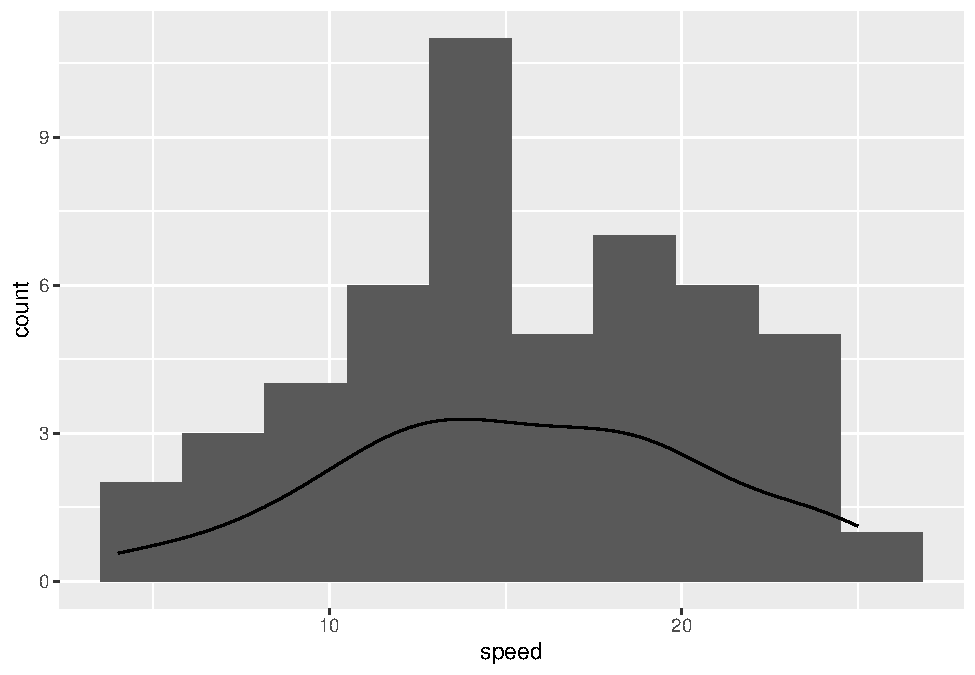
\includegraphics{R-with-Data-Science_files/figure-latex/unnamed-chunk-55-1.pdf}

\begin{Shaded}
\begin{Highlighting}[]
\FunctionTok{hist}\NormalTok{(}\FunctionTok{table}\NormalTok{(mo))}
\end{Highlighting}
\end{Shaded}

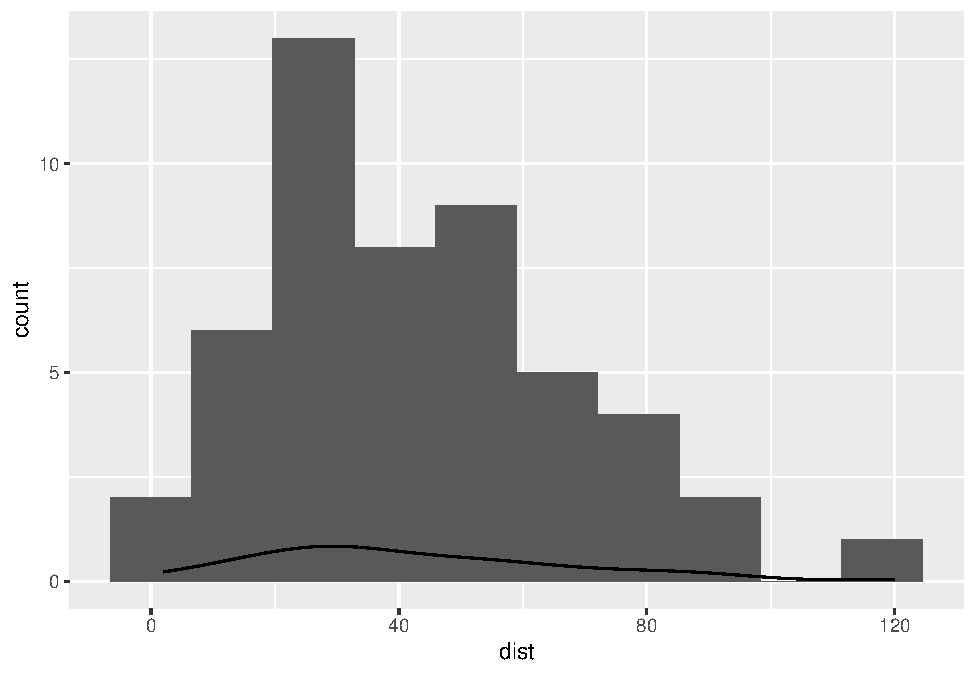
\includegraphics{R-with-Data-Science_files/figure-latex/unnamed-chunk-55-2.pdf}

\begin{Shaded}
\begin{Highlighting}[]
\FunctionTok{barplot}\NormalTok{(}\FunctionTok{prop.table}\NormalTok{(}\FunctionTok{table}\NormalTok{(mo)))}
\end{Highlighting}
\end{Shaded}

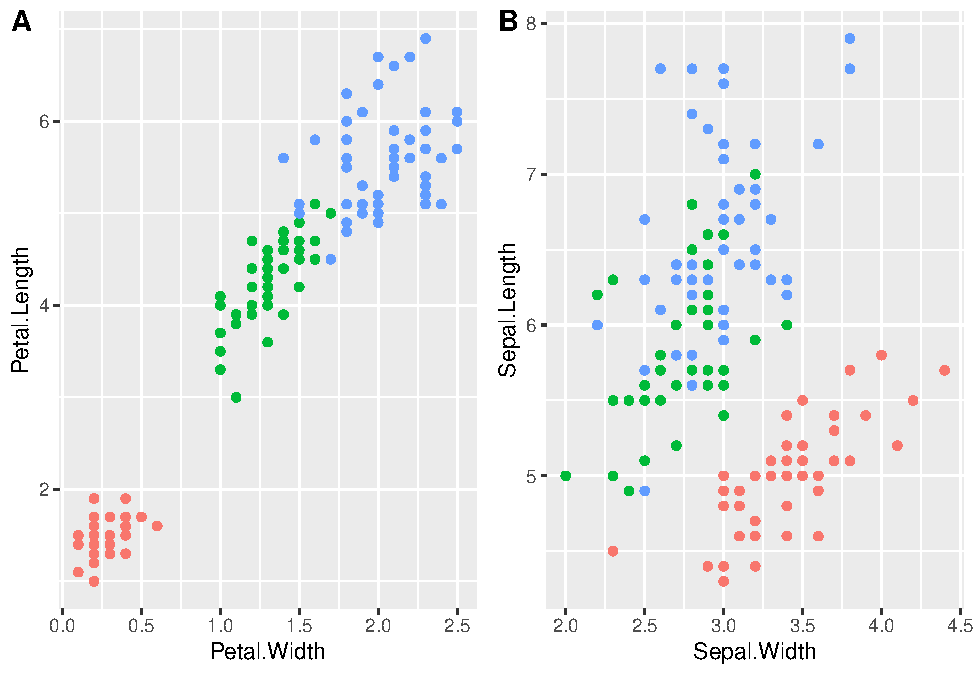
\includegraphics{R-with-Data-Science_files/figure-latex/unnamed-chunk-55-3.pdf}

\begin{Shaded}
\begin{Highlighting}[]
\FunctionTok{hist}\NormalTok{(}\FunctionTok{prop.table}\NormalTok{(}\FunctionTok{table}\NormalTok{(mo)))}
\end{Highlighting}
\end{Shaded}

\includegraphics{R-with-Data-Science_files/figure-latex/unnamed-chunk-55-4.pdf}

\begin{Shaded}
\begin{Highlighting}[]
\DocumentationTok{\#\#\# Pie Chart}
\FunctionTok{pie}\NormalTok{(}\FunctionTok{table}\NormalTok{(mo), }\AttributeTok{col =} \FunctionTok{c}\NormalTok{ (}\StringTok{"red"}\NormalTok{, }\StringTok{"green"}\NormalTok{, }\StringTok{"blue"}\NormalTok{, }\StringTok{"black"}\NormalTok{))}
\end{Highlighting}
\end{Shaded}

\includegraphics{R-with-Data-Science_files/figure-latex/unnamed-chunk-55-5.pdf}

\begin{Shaded}
\begin{Highlighting}[]
\FunctionTok{pie}\NormalTok{(}\FunctionTok{prop.table}\NormalTok{(}\FunctionTok{table}\NormalTok{(mo)), }\AttributeTok{col =} \FunctionTok{c}\NormalTok{(}\StringTok{"purple"}\NormalTok{, }\StringTok{"green"}\NormalTok{, }\StringTok{"red"}\NormalTok{, }\StringTok{"blue"}\NormalTok{))}
\end{Highlighting}
\end{Shaded}

\includegraphics{R-with-Data-Science_files/figure-latex/unnamed-chunk-55-6.pdf}

\begin{Shaded}
\begin{Highlighting}[]
\DocumentationTok{\#\#\# Contingency Matrix}
\NormalTok{g }\OtherTok{=} \FunctionTok{c}\NormalTok{(}\FunctionTok{rep}\NormalTok{(}\StringTok{"Male"}\NormalTok{,}\DecValTok{8}\NormalTok{), }\FunctionTok{rep}\NormalTok{(}\StringTok{"Female"}\NormalTok{,}\DecValTok{12}\NormalTok{))}
\NormalTok{g}
\end{Highlighting}
\end{Shaded}

\begin{verbatim}
##  [1] "Male"   "Male"   "Male"   "Male"   "Male"   "Male"   "Male"   "Male"  
##  [9] "Female" "Female" "Female" "Female" "Female" "Female" "Female" "Female"
## [17] "Female" "Female" "Female" "Female"
\end{verbatim}

\begin{Shaded}
\begin{Highlighting}[]
\NormalTok{mg }\OtherTok{=} \FunctionTok{table}\NormalTok{(mo,g)}
\NormalTok{mg}
\end{Highlighting}
\end{Shaded}

\begin{verbatim}
##        g
## mo      Female Male
##   bus        2    1
##   car        5    3
##   foot       2    0
##   metro      3    4
\end{verbatim}

\begin{Shaded}
\begin{Highlighting}[]
\NormalTok{gm }\OtherTok{=} \FunctionTok{data.frame}\NormalTok{(mo,g)}
\NormalTok{gm}
\end{Highlighting}
\end{Shaded}

\begin{verbatim}
##       mo      g
## 1    car   Male
## 2    car   Male
## 3    bus   Male
## 4  metro   Male
## 5  metro   Male
## 6    car   Male
## 7  metro   Male
## 8  metro   Male
## 9   foot Female
## 10   car Female
## 11  foot Female
## 12   bus Female
## 13   bus Female
## 14 metro Female
## 15 metro Female
## 16   car Female
## 17   car Female
## 18   car Female
## 19 metro Female
## 20   car Female
\end{verbatim}

\begin{Shaded}
\begin{Highlighting}[]
\FunctionTok{margin.table}\NormalTok{(mg, }\DecValTok{1}\NormalTok{)}
\end{Highlighting}
\end{Shaded}

\begin{verbatim}
## mo
##   bus   car  foot metro 
##     3     8     2     7
\end{verbatim}

\begin{Shaded}
\begin{Highlighting}[]
\FunctionTok{margin.table}\NormalTok{(mg,}\DecValTok{2}\NormalTok{)}
\end{Highlighting}
\end{Shaded}

\begin{verbatim}
## g
## Female   Male 
##     12      8
\end{verbatim}

\begin{Shaded}
\begin{Highlighting}[]
\FunctionTok{prop.table}\NormalTok{(mg)}
\end{Highlighting}
\end{Shaded}

\begin{verbatim}
##        g
## mo      Female Male
##   bus     0.10 0.05
##   car     0.25 0.15
##   foot    0.10 0.00
##   metro   0.15 0.20
\end{verbatim}

\begin{Shaded}
\begin{Highlighting}[]
\FunctionTok{prop.table}\NormalTok{(mg,}\DecValTok{1}\NormalTok{)}
\end{Highlighting}
\end{Shaded}

\begin{verbatim}
##        g
## mo         Female      Male
##   bus   0.6666667 0.3333333
##   car   0.6250000 0.3750000
##   foot  1.0000000 0.0000000
##   metro 0.4285714 0.5714286
\end{verbatim}

\begin{Shaded}
\begin{Highlighting}[]
\FunctionTok{prop.table}\NormalTok{(mg,}\DecValTok{2}\NormalTok{)}
\end{Highlighting}
\end{Shaded}

\begin{verbatim}
##        g
## mo         Female      Male
##   bus   0.1666667 0.1250000
##   car   0.4166667 0.3750000
##   foot  0.1666667 0.0000000
##   metro 0.2500000 0.5000000
\end{verbatim}

\begin{Shaded}
\begin{Highlighting}[]
\DocumentationTok{\#\#\# Stacked Bar Charts and Grouped Bar Charts}
\FunctionTok{barplot}\NormalTok{(mg, }\AttributeTok{col =} \FunctionTok{c}\NormalTok{(}\StringTok{"red"}\NormalTok{,}\StringTok{"blue"}\NormalTok{, }\StringTok{"pink"}\NormalTok{,}\StringTok{"green"}\NormalTok{))}
\end{Highlighting}
\end{Shaded}

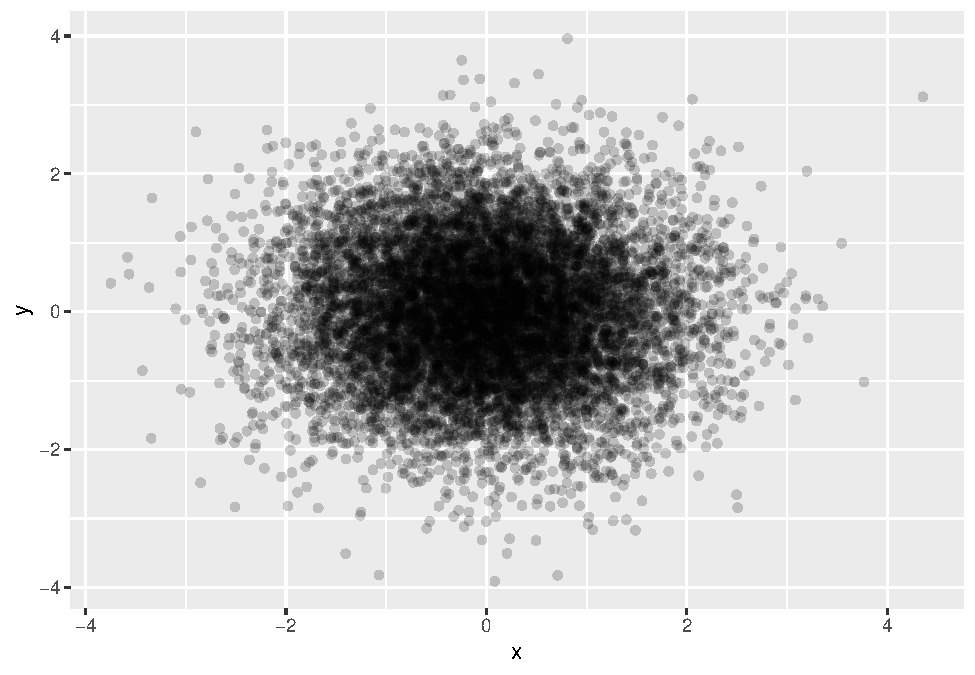
\includegraphics{R-with-Data-Science_files/figure-latex/unnamed-chunk-57-1.pdf}

\begin{Shaded}
\begin{Highlighting}[]
\FunctionTok{barplot}\NormalTok{(mg,}\AttributeTok{xlim=}\FunctionTok{c}\NormalTok{(}\DecValTok{0}\NormalTok{,}\DecValTok{2}\NormalTok{), }\AttributeTok{xlab=}\StringTok{"Gender"}\NormalTok{, }\AttributeTok{length=}\FunctionTok{levels}\NormalTok{(mo), }\AttributeTok{col =} \FunctionTok{c}\NormalTok{(}\StringTok{"red"}\NormalTok{,}\StringTok{"blue"}\NormalTok{, }\StringTok{"pink"}\NormalTok{,}\StringTok{"green"}\NormalTok{))}
\end{Highlighting}
\end{Shaded}

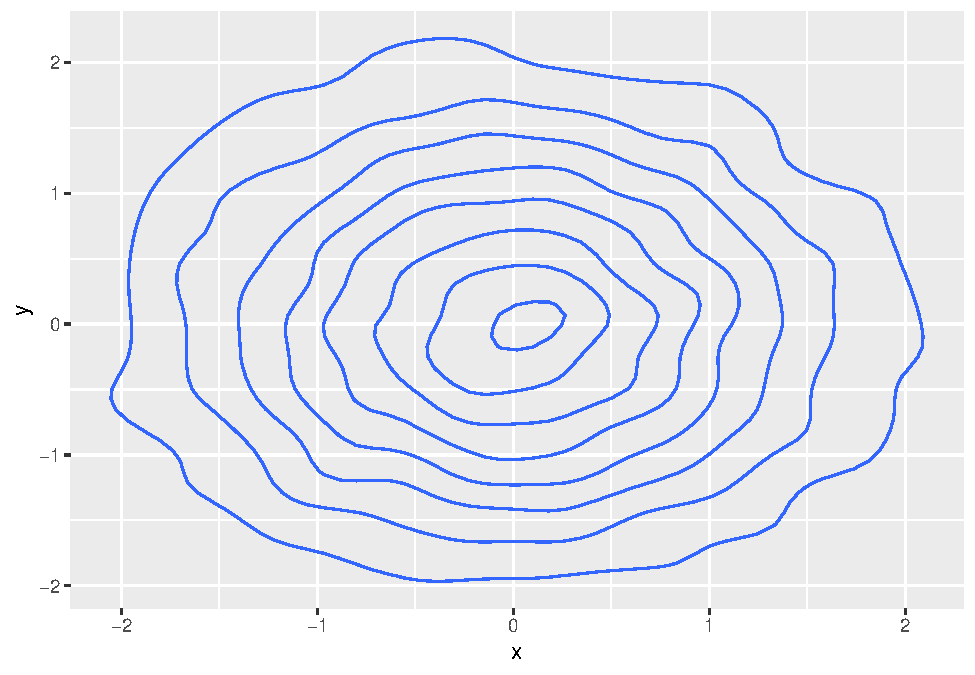
\includegraphics{R-with-Data-Science_files/figure-latex/unnamed-chunk-57-2.pdf}

\begin{Shaded}
\begin{Highlighting}[]
\FunctionTok{barplot}\NormalTok{(mg,}\AttributeTok{xlim=}\FunctionTok{c}\NormalTok{(}\DecValTok{0}\NormalTok{,}\DecValTok{2}\NormalTok{), }\AttributeTok{xlab=}\StringTok{"Transportation"}\NormalTok{, }\AttributeTok{length=}\FunctionTok{levels}\NormalTok{(g), }\AttributeTok{col =} \FunctionTok{c}\NormalTok{(}\StringTok{"red"}\NormalTok{,}\StringTok{"blue"}\NormalTok{, }\StringTok{"pink"}\NormalTok{,}\StringTok{"green"}\NormalTok{))}
\end{Highlighting}
\end{Shaded}

\includegraphics{R-with-Data-Science_files/figure-latex/unnamed-chunk-57-3.pdf}

\begin{Shaded}
\begin{Highlighting}[]
\FunctionTok{barplot}\NormalTok{(}\FunctionTok{prop.table}\NormalTok{(mg,}\DecValTok{1}\NormalTok{), }\AttributeTok{width=}\FloatTok{0.25}\NormalTok{, }\AttributeTok{xlim=}\FunctionTok{c}\NormalTok{(}\DecValTok{0}\NormalTok{,}\DecValTok{3}\NormalTok{), }\AttributeTok{ylim=}\FunctionTok{c}\NormalTok{(}\DecValTok{0}\NormalTok{,}\DecValTok{1}\NormalTok{), }\AttributeTok{xlab=}\StringTok{"Gender"}\NormalTok{, }\AttributeTok{legend=}\FunctionTok{levels}\NormalTok{(mo), }\AttributeTok{beside=}\NormalTok{T, }\AttributeTok{col =} \FunctionTok{c}\NormalTok{(}\StringTok{"red"}\NormalTok{,}\StringTok{"blue"}\NormalTok{, }\StringTok{"pink"}\NormalTok{,}\StringTok{"green"}\NormalTok{))}
\end{Highlighting}
\end{Shaded}

\includegraphics{R-with-Data-Science_files/figure-latex/unnamed-chunk-57-4.pdf}

\begin{Shaded}
\begin{Highlighting}[]
\NormalTok{mg }\OtherTok{=} \FunctionTok{table}\NormalTok{(g,mo)}
\FunctionTok{barplot}\NormalTok{(}\FunctionTok{prop.table}\NormalTok{(mg,}\DecValTok{2}\NormalTok{), }\AttributeTok{width=}\FloatTok{0.25}\NormalTok{, }\AttributeTok{xlim=}\FunctionTok{c}\NormalTok{(}\DecValTok{0}\NormalTok{,}\DecValTok{3}\NormalTok{), }\AttributeTok{ylim=}\FunctionTok{c}\NormalTok{(}\DecValTok{0}\NormalTok{,}\DecValTok{1}\NormalTok{), }\AttributeTok{xlab=}\StringTok{"Transportation"}\NormalTok{, }\AttributeTok{legend=}\FunctionTok{levels}\NormalTok{(g), }\AttributeTok{beside=}\NormalTok{T, }\AttributeTok{col=} \FunctionTok{c}\NormalTok{(}\StringTok{"red"}\NormalTok{, }\StringTok{"green"}\NormalTok{))}
\end{Highlighting}
\end{Shaded}

\includegraphics{R-with-Data-Science_files/figure-latex/unnamed-chunk-57-5.pdf}

\begin{Shaded}
\begin{Highlighting}[]
\NormalTok{xo }\OtherTok{=} \FunctionTok{c}\NormalTok{(}\DecValTok{10}\NormalTok{, }\DecValTok{10}\NormalTok{, }\DecValTok{5}\NormalTok{, }\DecValTok{9}\NormalTok{, }\DecValTok{7}\NormalTok{, }\DecValTok{6}\NormalTok{,}\DecValTok{8}\NormalTok{,}\DecValTok{6}\NormalTok{,}\DecValTok{5}\NormalTok{,}\DecValTok{8}\NormalTok{, }\DecValTok{10}\NormalTok{, }\DecValTok{7}\NormalTok{, }\DecValTok{7}\NormalTok{,}\DecValTok{8}\NormalTok{, }\DecValTok{5}\NormalTok{, }\DecValTok{6}\NormalTok{,}\DecValTok{4}\NormalTok{,}\DecValTok{7}\NormalTok{,}\DecValTok{9}\NormalTok{,}\DecValTok{7}\NormalTok{, }\DecValTok{4}\NormalTok{,}\DecValTok{8}\NormalTok{, }\DecValTok{10}\NormalTok{,}\DecValTok{10}\NormalTok{, }\DecValTok{7}\NormalTok{,}\DecValTok{4}\NormalTok{,}\DecValTok{9}\NormalTok{,}\DecValTok{5}\NormalTok{,}\DecValTok{8}\NormalTok{,}\DecValTok{9}\NormalTok{)}
\FunctionTok{table}\NormalTok{(xo)}
\end{Highlighting}
\end{Shaded}

\begin{verbatim}
## xo
##  4  5  6  7  8  9 10 
##  3  4  3  6  5  4  5
\end{verbatim}

\begin{Shaded}
\begin{Highlighting}[]
\FunctionTok{data.frame}\NormalTok{(xo)}
\end{Highlighting}
\end{Shaded}

\begin{verbatim}
##    xo
## 1  10
## 2  10
## 3   5
## 4   9
## 5   7
## 6   6
## 7   8
## 8   6
## 9   5
## 10  8
## 11 10
## 12  7
## 13  7
## 14  8
## 15  5
## 16  6
## 17  4
## 18  7
## 19  9
## 20  7
## 21  4
## 22  8
## 23 10
## 24 10
## 25  7
## 26  4
## 27  9
## 28  5
## 29  8
## 30  9
\end{verbatim}

\begin{Shaded}
\begin{Highlighting}[]
\FunctionTok{prop.table}\NormalTok{(}\FunctionTok{table}\NormalTok{(xo))}
\end{Highlighting}
\end{Shaded}

\begin{verbatim}
## xo
##         4         5         6         7         8         9        10 
## 0.1000000 0.1333333 0.1000000 0.2000000 0.1666667 0.1333333 0.1666667
\end{verbatim}

\begin{Shaded}
\begin{Highlighting}[]
\NormalTok{?prop.table}

\DocumentationTok{\#\#\# Histograms}
\FunctionTok{hist}\NormalTok{(xo, }\AttributeTok{col =} \FunctionTok{c}\NormalTok{(}\StringTok{"red"}\NormalTok{,}\StringTok{"blue"}\NormalTok{, }\StringTok{"pink"}\NormalTok{,}\StringTok{"green"}\NormalTok{))}
\end{Highlighting}
\end{Shaded}

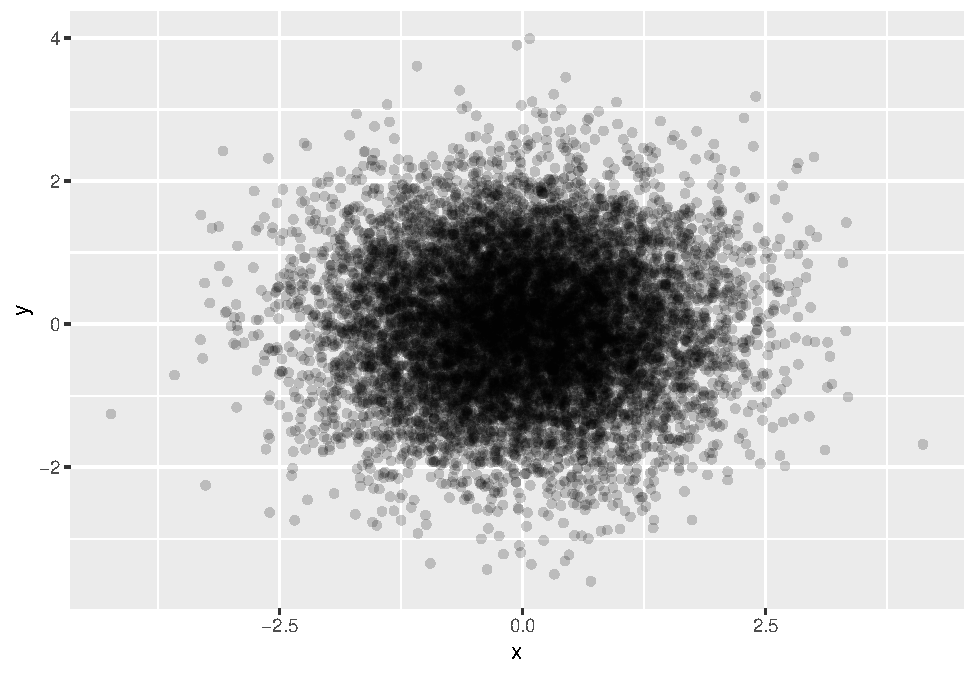
\includegraphics{R-with-Data-Science_files/figure-latex/unnamed-chunk-58-1.pdf}

\begin{Shaded}
\begin{Highlighting}[]
\FunctionTok{hist}\NormalTok{(xo, }\AttributeTok{nclass=}\DecValTok{3}\NormalTok{, }\AttributeTok{col =} \FunctionTok{c}\NormalTok{(}\StringTok{"red"}\NormalTok{,}\StringTok{"blue"}\NormalTok{, }\StringTok{"pink"}\NormalTok{,}\StringTok{"green"}\NormalTok{))}
\end{Highlighting}
\end{Shaded}

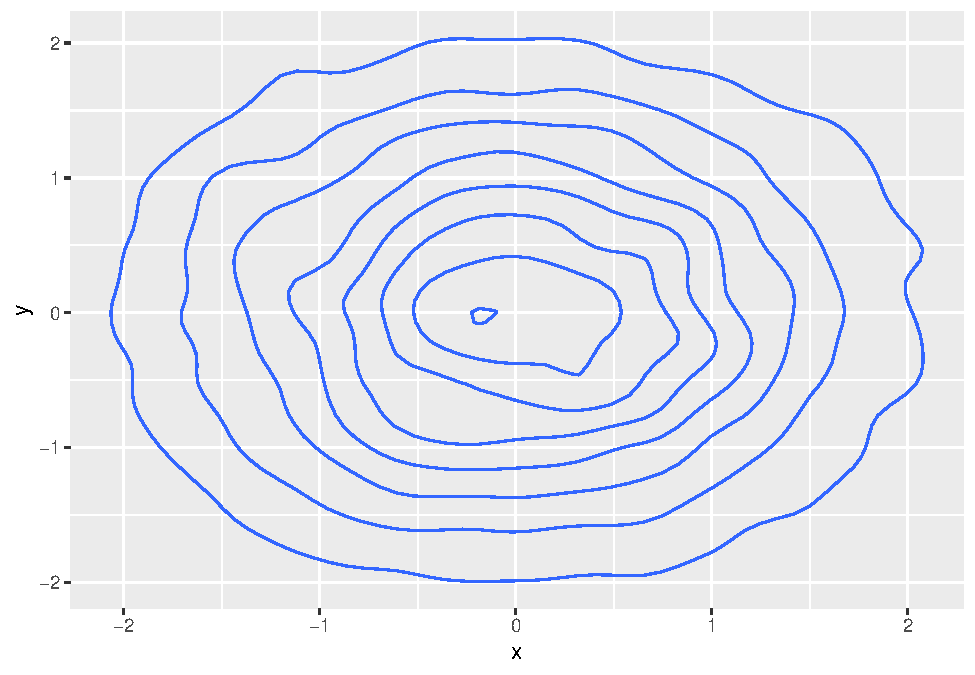
\includegraphics{R-with-Data-Science_files/figure-latex/unnamed-chunk-58-2.pdf}

\begin{Shaded}
\begin{Highlighting}[]
\NormalTok{wo }\OtherTok{=} \FunctionTok{c}\NormalTok{ (}\DecValTok{1950}\NormalTok{, }\DecValTok{2090}\NormalTok{, }\DecValTok{2700}\NormalTok{, }\DecValTok{3350}\NormalTok{, }\DecValTok{4200}\NormalTok{, }\DecValTok{3720}\NormalTok{, }\DecValTok{4400}\NormalTok{, }\DecValTok{2980}\NormalTok{, }\DecValTok{3850}\NormalTok{, }\DecValTok{4550}\NormalTok{, }\DecValTok{3050}\NormalTok{, }\DecValTok{2350}\NormalTok{, }\DecValTok{1850}\NormalTok{, }\DecValTok{2820}\NormalTok{, }\DecValTok{3670}\NormalTok{, }\DecValTok{2950}\NormalTok{, }\DecValTok{3750}\NormalTok{, }\DecValTok{1850}\NormalTok{, }\DecValTok{2420}\NormalTok{, }\DecValTok{3150}\NormalTok{, }\DecValTok{3000}\NormalTok{, }\DecValTok{3470}\NormalTok{, }\DecValTok{3920}\NormalTok{, }\DecValTok{3100}\NormalTok{, }\DecValTok{2400}\NormalTok{, }\DecValTok{2900}\NormalTok{, }\DecValTok{2650}\NormalTok{, }\DecValTok{3450}\NormalTok{, }\DecValTok{3650}\NormalTok{, }\DecValTok{4020}\NormalTok{, }\DecValTok{4450}\NormalTok{, }\DecValTok{3120}\NormalTok{, }\DecValTok{3660}\NormalTok{, }\DecValTok{3070}\NormalTok{, }\DecValTok{3550}\NormalTok{, }\DecValTok{2020}\NormalTok{, }\DecValTok{3500}\NormalTok{, }\DecValTok{2500}\NormalTok{, }\DecValTok{3780}\NormalTok{, }\DecValTok{3940}\NormalTok{, }\DecValTok{3540}\NormalTok{, }\DecValTok{2800}\NormalTok{, }\DecValTok{4450}\NormalTok{, }\DecValTok{1950}\NormalTok{, }\DecValTok{3020}\NormalTok{, }\DecValTok{2800}\NormalTok{, }\DecValTok{3500}\NormalTok{, }\DecValTok{1480}\NormalTok{, }\DecValTok{4495}\NormalTok{,}\DecValTok{2850}\NormalTok{, }\DecValTok{3100}\NormalTok{, }\DecValTok{2250}\NormalTok{,}\DecValTok{3300}\NormalTok{, }\DecValTok{4100}\NormalTok{, }\DecValTok{3220}\NormalTok{, }\DecValTok{3600}\NormalTok{,}\DecValTok{2130}\NormalTok{, }\DecValTok{4020}\NormalTok{, }\DecValTok{4075}\NormalTok{)}
\FunctionTok{hist}\NormalTok{(wo, }\AttributeTok{col =} \FunctionTok{c}\NormalTok{(}\StringTok{"red"}\NormalTok{,}\StringTok{"blue"}\NormalTok{, }\StringTok{"pink"}\NormalTok{,}\StringTok{"green"}\NormalTok{))}
\end{Highlighting}
\end{Shaded}

\includegraphics{R-with-Data-Science_files/figure-latex/unnamed-chunk-58-3.pdf}

\begin{Shaded}
\begin{Highlighting}[]
\FunctionTok{hist}\NormalTok{(wo, }\AttributeTok{nclass=}\DecValTok{4}\NormalTok{, }\AttributeTok{col =} \FunctionTok{c}\NormalTok{(}\StringTok{"red"}\NormalTok{,}\StringTok{"blue"}\NormalTok{, }\StringTok{"pink"}\NormalTok{,}\StringTok{"green"}\NormalTok{))}
\end{Highlighting}
\end{Shaded}

\includegraphics{R-with-Data-Science_files/figure-latex/unnamed-chunk-58-4.pdf}

\begin{Shaded}
\begin{Highlighting}[]
\FunctionTok{hist}\NormalTok{(wo, }\AttributeTok{breaks=} \FunctionTok{seq}\NormalTok{(}\AttributeTok{from =} \DecValTok{1000}\NormalTok{, }\AttributeTok{to=}\DecValTok{5000}\NormalTok{, }\AttributeTok{by=}\DecValTok{300}\NormalTok{), }\AttributeTok{col =} \FunctionTok{c}\NormalTok{(}\StringTok{"red"}\NormalTok{,}\StringTok{"blue"}\NormalTok{, }\StringTok{"pink"}\NormalTok{,}\StringTok{"green"}\NormalTok{))}
\end{Highlighting}
\end{Shaded}

\includegraphics{R-with-Data-Science_files/figure-latex/unnamed-chunk-58-5.pdf}

\begin{Shaded}
\begin{Highlighting}[]
\FunctionTok{hist}\NormalTok{(wo, }\AttributeTok{probability=}\NormalTok{T, }\AttributeTok{col =} \FunctionTok{c}\NormalTok{(}\StringTok{"red"}\NormalTok{,}\StringTok{"blue"}\NormalTok{, }\StringTok{"pink"}\NormalTok{,}\StringTok{"green"}\NormalTok{))}
\FunctionTok{rug}\NormalTok{(}\FunctionTok{jitter}\NormalTok{(wo))}
\end{Highlighting}
\end{Shaded}

\includegraphics{R-with-Data-Science_files/figure-latex/unnamed-chunk-58-6.pdf}

\begin{Shaded}
\begin{Highlighting}[]
\DocumentationTok{\#\#\# Frequency Polygon}
\NormalTok{temp }\OtherTok{=} \FunctionTok{hist}\NormalTok{(wo, }\AttributeTok{col =} \FunctionTok{c}\NormalTok{(}\StringTok{"red"}\NormalTok{,}\StringTok{"blue"}\NormalTok{, }\StringTok{"purple"}\NormalTok{,}\StringTok{"green"}\NormalTok{))}
\NormalTok{temp}
\end{Highlighting}
\end{Shaded}

\begin{verbatim}
## $breaks
## [1] 1000 1500 2000 2500 3000 3500 4000 4500 5000
## 
## $counts
## [1]  1  4  8 10 14 12  9  1
## 
## $density
## [1] 3.389831e-05 1.355932e-04 2.711864e-04 3.389831e-04 4.745763e-04
## [6] 4.067797e-04 3.050847e-04 3.389831e-05
## 
## $mids
## [1] 1250 1750 2250 2750 3250 3750 4250 4750
## 
## $xname
## [1] "wo"
## 
## $equidist
## [1] TRUE
## 
## attr(,"class")
## [1] "histogram"
\end{verbatim}

\begin{Shaded}
\begin{Highlighting}[]
\FunctionTok{lines}\NormalTok{(}\FunctionTok{c}\NormalTok{(}\FunctionTok{min}\NormalTok{(temp}\SpecialCharTok{$}\NormalTok{breaks), (temp}\SpecialCharTok{$}\NormalTok{mids),}\FunctionTok{max}\NormalTok{(temp}\SpecialCharTok{$}\NormalTok{breaks)), }\FunctionTok{c}\NormalTok{(}\DecValTok{0}\NormalTok{,temp}\SpecialCharTok{$}\NormalTok{counts,}\DecValTok{0}\NormalTok{),}\AttributeTok{type=}\StringTok{"l"}\NormalTok{)}
\end{Highlighting}
\end{Shaded}

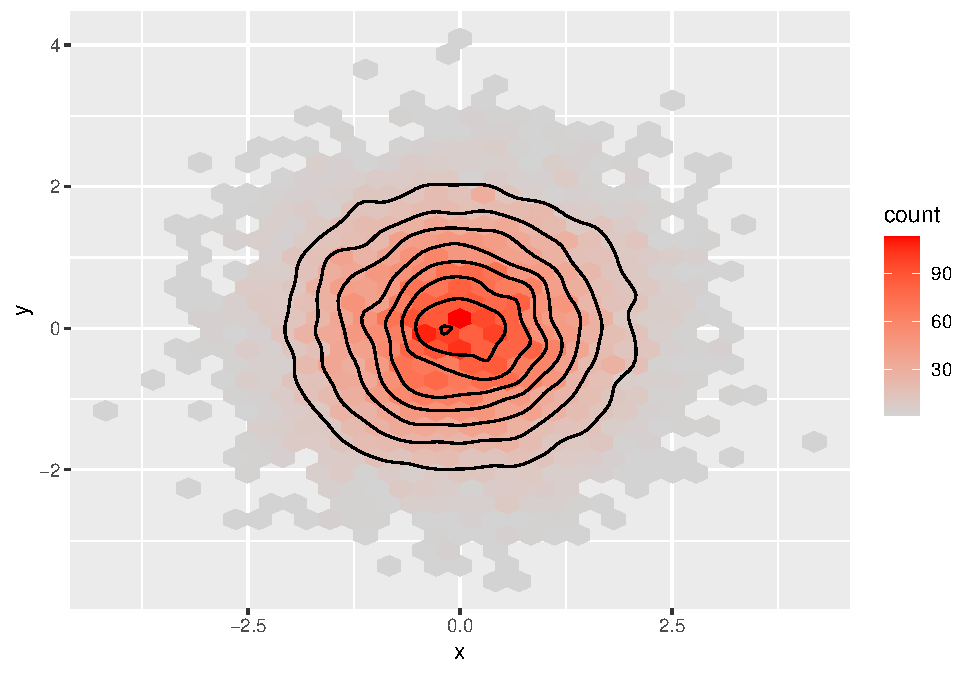
\includegraphics{R-with-Data-Science_files/figure-latex/unnamed-chunk-59-1.pdf}

\begin{Shaded}
\begin{Highlighting}[]
\FunctionTok{boxplot}\NormalTok{(wo, }\AttributeTok{horizontal =}\NormalTok{ T, }\AttributeTok{col =} \FunctionTok{c}\NormalTok{(}\StringTok{"red"}\NormalTok{))}
\end{Highlighting}
\end{Shaded}

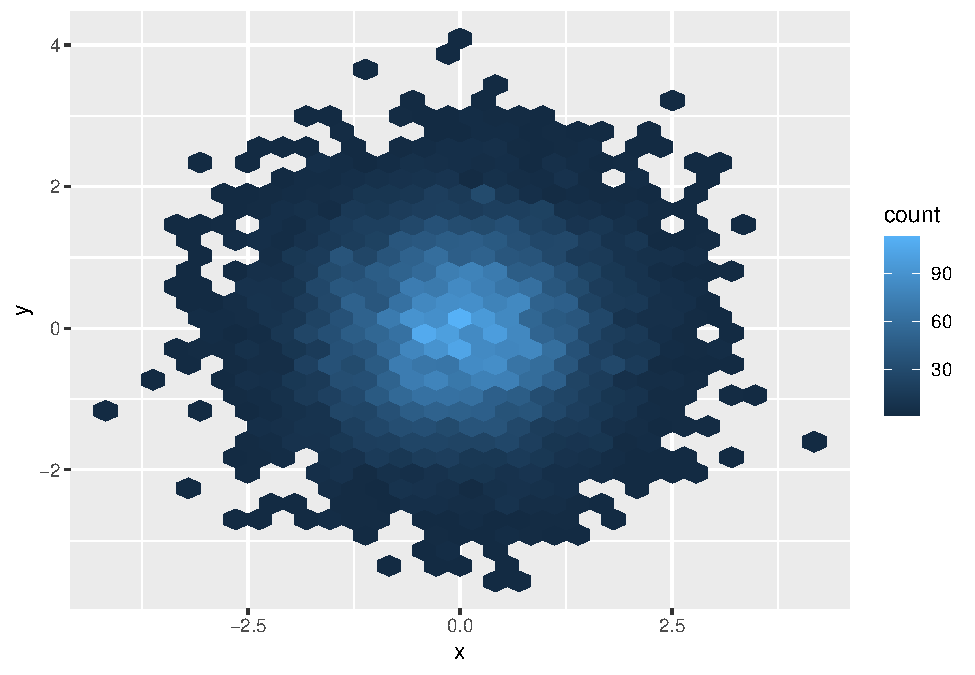
\includegraphics{R-with-Data-Science_files/figure-latex/unnamed-chunk-59-2.pdf}

\begin{Shaded}
\begin{Highlighting}[]
\FunctionTok{boxplot}\NormalTok{(wo, }\AttributeTok{vertical =}\NormalTok{ T, }\AttributeTok{col =} \FunctionTok{c}\NormalTok{(}\StringTok{"red"}\NormalTok{))}
\end{Highlighting}
\end{Shaded}

\includegraphics{R-with-Data-Science_files/figure-latex/unnamed-chunk-59-3.pdf}

\begin{Shaded}
\begin{Highlighting}[]
\FunctionTok{fivenum}\NormalTok{(wo)}
\end{Highlighting}
\end{Shaded}

\begin{verbatim}
## [1] 1480 2750 3150 3735 4550
\end{verbatim}

\begin{Shaded}
\begin{Highlighting}[]
\FunctionTok{summary}\NormalTok{(wo)}
\end{Highlighting}
\end{Shaded}

\begin{verbatim}
##    Min. 1st Qu.  Median    Mean 3rd Qu.    Max. 
##    1480    2750    3150    3195    3735    4550
\end{verbatim}

\begin{Shaded}
\begin{Highlighting}[]
\NormalTok{?fivenum}
\end{Highlighting}
\end{Shaded}

\begin{Shaded}
\begin{Highlighting}[]
\NormalTok{w1 }\OtherTok{=} \FunctionTok{c}\NormalTok{(}\DecValTok{1950}\NormalTok{, }\DecValTok{2090}\NormalTok{, }\DecValTok{2700}\NormalTok{, }\DecValTok{3350}\NormalTok{, }\DecValTok{4200}\NormalTok{, }\DecValTok{3720}\NormalTok{, }\DecValTok{4400}\NormalTok{, }\DecValTok{2980}\NormalTok{, }\DecValTok{3850}\NormalTok{, }\DecValTok{4550}\NormalTok{, }\DecValTok{3050}\NormalTok{, }\DecValTok{2350}\NormalTok{,}\DecValTok{1850}\NormalTok{, }\DecValTok{2820}\NormalTok{, }\DecValTok{3670}\NormalTok{, }\DecValTok{2950}\NormalTok{, }\DecValTok{3750}\NormalTok{, }\DecValTok{1850}\NormalTok{, }\DecValTok{2420}\NormalTok{,}\DecValTok{3150}\NormalTok{, }\DecValTok{3000}\NormalTok{, }\DecValTok{3470}\NormalTok{, }\DecValTok{3920}\NormalTok{, }\DecValTok{3100}\NormalTok{, }\DecValTok{2400}\NormalTok{, }\DecValTok{2900}\NormalTok{, }\DecValTok{2650}\NormalTok{, }\DecValTok{3450}\NormalTok{, }\DecValTok{3650}\NormalTok{, }\DecValTok{4020}\NormalTok{)}
\FunctionTok{fivenum}\NormalTok{(w1)}
\end{Highlighting}
\end{Shaded}

\begin{verbatim}
## [1] 1850 2650 3075 3720 4550
\end{verbatim}

\begin{Shaded}
\begin{Highlighting}[]
\NormalTok{w2 }\OtherTok{=} \FunctionTok{c}\NormalTok{(}\DecValTok{4450}\NormalTok{, }\DecValTok{3120}\NormalTok{, }\DecValTok{3660}\NormalTok{, }\DecValTok{3070}\NormalTok{, }\DecValTok{3550}\NormalTok{, }\DecValTok{2020}\NormalTok{, }\DecValTok{3500}\NormalTok{, }\DecValTok{2500}\NormalTok{, }\DecValTok{3780}\NormalTok{, }\DecValTok{3940}\NormalTok{, }\DecValTok{3340}\NormalTok{, }\DecValTok{2800}\NormalTok{, }\DecValTok{2850}\NormalTok{, }\DecValTok{4450}\NormalTok{, }\DecValTok{1950}\NormalTok{,}\DecValTok{3020}\NormalTok{,}\DecValTok{2800}\NormalTok{,}\DecValTok{3500}\NormalTok{,}\DecValTok{1480}\NormalTok{,}\DecValTok{4495}\NormalTok{,}\DecValTok{2850}\NormalTok{,}\DecValTok{3100}\NormalTok{,}\DecValTok{2250}\NormalTok{,}\DecValTok{3300}\NormalTok{,}\DecValTok{4100}\NormalTok{,}\DecValTok{3220}\NormalTok{,}\DecValTok{3600}\NormalTok{,}\DecValTok{2130}\NormalTok{,}\DecValTok{4020}\NormalTok{,}\DecValTok{4075}\NormalTok{)}
\FunctionTok{fivenum}\NormalTok{(w2)}
\end{Highlighting}
\end{Shaded}

\begin{verbatim}
## [1] 1480 2800 3260 3780 4495
\end{verbatim}

\begin{Shaded}
\begin{Highlighting}[]
\FunctionTok{boxplot}\NormalTok{(w1, w2, }\AttributeTok{names=}\FunctionTok{c}\NormalTok{(}\StringTok{"sample 1"}\NormalTok{, }\StringTok{"sample 2"}\NormalTok{), }\AttributeTok{col =} \FunctionTok{c}\NormalTok{(}\StringTok{"purple"}\NormalTok{, }\StringTok{"yellow"}\NormalTok{ ))}
\end{Highlighting}
\end{Shaded}

\includegraphics{R-with-Data-Science_files/figure-latex/unnamed-chunk-60-1.pdf}

\begin{Shaded}
\begin{Highlighting}[]
\CommentTok{\# Classification and Prediction}

\NormalTok{computeCost }\OtherTok{\textless{}{-}} \ControlFlowTok{function}\NormalTok{(X, y, th)\{}
\NormalTok{m }\OtherTok{\textless{}{-}} \FunctionTok{length}\NormalTok{(y)}
\FunctionTok{return}\NormalTok{(}\DecValTok{1}\SpecialCharTok{/}\NormalTok{(}\DecValTok{2}\SpecialCharTok{*}\NormalTok{m) }\SpecialCharTok{*} \FunctionTok{sum}\NormalTok{((X}\SpecialCharTok{\%*\%}\NormalTok{th }\SpecialCharTok{{-}}\NormalTok{ y)}\SpecialCharTok{\^{}}\DecValTok{2}\NormalTok{))}
\NormalTok{\}}

\FunctionTok{computeCost}\NormalTok{(}\DecValTok{5}\NormalTok{,}\DecValTok{6}\NormalTok{,}\DecValTok{7}\NormalTok{)}
\end{Highlighting}
\end{Shaded}

\begin{verbatim}
## [1] 420.5
\end{verbatim}

\begin{Shaded}
\begin{Highlighting}[]
\NormalTok{grad\_desc }\OtherTok{\textless{}{-}} \ControlFlowTok{function}\NormalTok{(X, y, theta,alpha, lambda, num\_iters)\{}
\NormalTok{m }\OtherTok{\textless{}{-}} \FunctionTok{length}\NormalTok{(y)}
\NormalTok{F\_history }\OtherTok{\textless{}{-}} \FunctionTok{c}\NormalTok{(}\FunctionTok{rep}\NormalTok{(}\DecValTok{0}\NormalTok{, num\_iters))}

\ControlFlowTok{for}\NormalTok{ (iter }\ControlFlowTok{in} \FunctionTok{c}\NormalTok{(}\DecValTok{1}\SpecialCharTok{:}\NormalTok{num\_iters))\{}
\NormalTok{  temp }\OtherTok{\textless{}{-}} \FunctionTok{vector}\NormalTok{()}
\NormalTok{  temp }\OtherTok{\textless{}{-}}\NormalTok{ theta }\SpecialCharTok{*}\NormalTok{ (}\DecValTok{1} \SpecialCharTok{{-}}\NormalTok{ ((alpha}\SpecialCharTok{*}\NormalTok{lambda)}\SpecialCharTok{/}\NormalTok{m)) }\SpecialCharTok{{-}}\NormalTok{ alpha}\SpecialCharTok{*}\NormalTok{(}\DecValTok{1}\SpecialCharTok{/}\NormalTok{m) }\SpecialCharTok{*}\NormalTok{   (}\FunctionTok{t}\NormalTok{(X) }\SpecialCharTok{\%*\%}\NormalTok{ (X }\SpecialCharTok{\%*\%}\NormalTok{ theta }\SpecialCharTok{{-}}\NormalTok{ y))}
\NormalTok{  theta }\OtherTok{\textless{}{-}}\NormalTok{ temp}
\NormalTok{  F\_history[iter] }\OtherTok{\textless{}{-}} \FunctionTok{computeCost}\NormalTok{(X, y, theta)}
\NormalTok{\}}
\FunctionTok{print}\NormalTok{(F\_history[num\_iters])}
\FunctionTok{return}\NormalTok{(}\FunctionTok{list}\NormalTok{(}\StringTok{"theta"} \OtherTok{=}\NormalTok{ theta, }\StringTok{"F\_history"} \OtherTok{=}\NormalTok{ F\_history))}
\NormalTok{\}}

\FunctionTok{grad\_desc}\NormalTok{(}\DecValTok{2}\NormalTok{,}\DecValTok{3}\NormalTok{,}\DecValTok{5}\NormalTok{,}\FloatTok{0.1}\NormalTok{,}\FloatTok{7.5}\NormalTok{,}\DecValTok{2}\NormalTok{)}
\end{Highlighting}
\end{Shaded}

\begin{verbatim}
## [1] 1.540012
\end{verbatim}

\begin{verbatim}
## $theta
##        [,1]
## [1,] 0.6225
## 
## $F_history
## [1] 5.445000 1.540012
\end{verbatim}

\begin{Shaded}
\begin{Highlighting}[]
\DocumentationTok{\#\#\# Clustering}
\NormalTok{iris\_new }\OtherTok{\textless{}{-}}\NormalTok{ iris}
\DocumentationTok{\#\#\# iris\_new}
\NormalTok{iris\_new}\SpecialCharTok{$}\NormalTok{Species }\OtherTok{\textless{}{-}} \ConstantTok{NULL}
\NormalTok{kc }\OtherTok{\textless{}{-}} \FunctionTok{kmeans}\NormalTok{(iris\_new, }\DecValTok{3}\NormalTok{)}
\FunctionTok{table}\NormalTok{(iris}\SpecialCharTok{$}\NormalTok{Species, kc}\SpecialCharTok{$}\NormalTok{cluster)}
\end{Highlighting}
\end{Shaded}

\begin{verbatim}
##             
##               1  2  3
##   setosa     50  0  0
##   versicolor  0 48  2
##   virginica   0 14 36
\end{verbatim}

\begin{Shaded}
\begin{Highlighting}[]
\FunctionTok{plot}\NormalTok{(iris\_new[}\FunctionTok{c}\NormalTok{(}\StringTok{"Sepal.Length"}\NormalTok{, }\StringTok{"Sepal.Width"}\NormalTok{)], }\AttributeTok{col =}\NormalTok{ kc}\SpecialCharTok{$}\NormalTok{cluster)}
\FunctionTok{points}\NormalTok{(kc}\SpecialCharTok{$}\NormalTok{centers[,}\FunctionTok{c}\NormalTok{(}\StringTok{"Sepal.Length"}\NormalTok{,}\StringTok{"Sepal.Width"}\NormalTok{)], }\AttributeTok{col =} \DecValTok{1}\SpecialCharTok{:}\DecValTok{3}\NormalTok{, }\AttributeTok{pch=}\DecValTok{8}\NormalTok{, }\AttributeTok{cex=}\DecValTok{2}\NormalTok{)}
\end{Highlighting}
\end{Shaded}

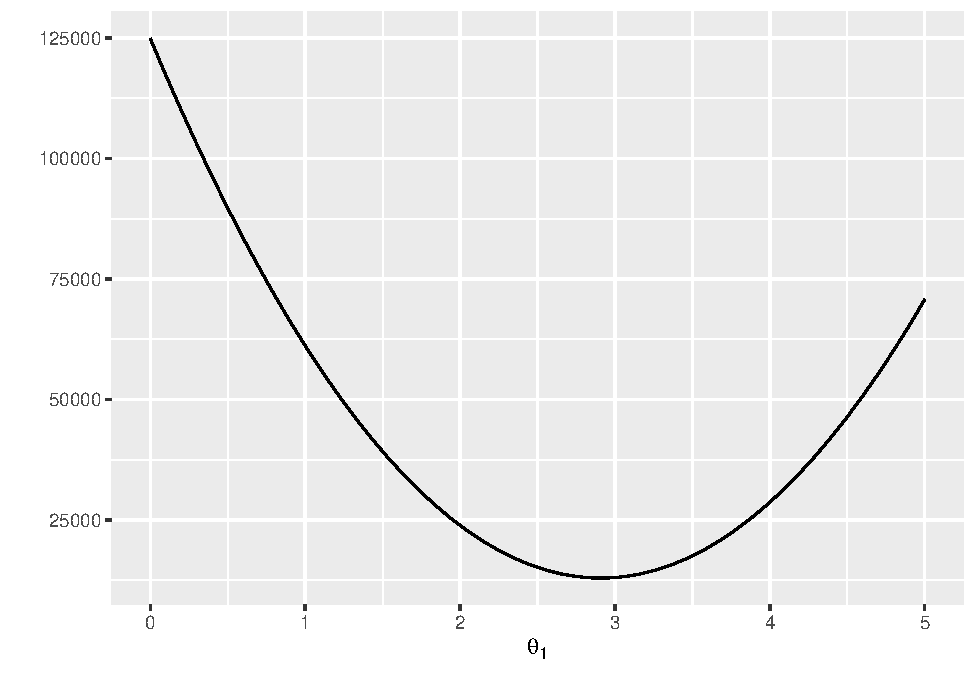
\includegraphics{R-with-Data-Science_files/figure-latex/unnamed-chunk-62-1.pdf}

\begin{Shaded}
\begin{Highlighting}[]
\FunctionTok{plot}\NormalTok{(iris\_new[}\FunctionTok{c}\NormalTok{(}\StringTok{"Petal.Length"}\NormalTok{, }\StringTok{"Petal.Width"}\NormalTok{)], }\AttributeTok{col =}\NormalTok{ kc}\SpecialCharTok{$}\NormalTok{cluster)}
\FunctionTok{points}\NormalTok{(kc}\SpecialCharTok{$}\NormalTok{centers[,}\FunctionTok{c}\NormalTok{(}\StringTok{"Petal.Length"}\NormalTok{,}\StringTok{"Petal.Width"}\NormalTok{)], }\AttributeTok{col=}\DecValTok{1}\SpecialCharTok{:}\DecValTok{3}\NormalTok{, }\AttributeTok{pch=}\DecValTok{8}\NormalTok{, }\AttributeTok{cex=}\DecValTok{2}\NormalTok{)}
\end{Highlighting}
\end{Shaded}

\includegraphics{R-with-Data-Science_files/figure-latex/unnamed-chunk-62-2.pdf}

\begin{Shaded}
\begin{Highlighting}[]
\FunctionTok{data}\NormalTok{(iris)}
\FunctionTok{set.seed}\NormalTok{(}\DecValTok{500}\NormalTok{)}
\NormalTok{idx }\OtherTok{\textless{}{-}} \FunctionTok{sample}\NormalTok{(}\DecValTok{1}\SpecialCharTok{:}\FunctionTok{dim}\NormalTok{(iris)[}\DecValTok{1}\NormalTok{], }\DecValTok{40}\NormalTok{)}
\NormalTok{iris\_Sample }\OtherTok{\textless{}{-}}\NormalTok{ iris[idx,]}
\NormalTok{iris\_Sample}\SpecialCharTok{$}\NormalTok{Species }\OtherTok{\textless{}{-}} \ConstantTok{NULL}
\NormalTok{hc }\OtherTok{\textless{}{-}} \FunctionTok{hclust}\NormalTok{(}\FunctionTok{dist}\NormalTok{(iris\_Sample), }\AttributeTok{method =} \StringTok{"single"}\NormalTok{)}
\FunctionTok{plot}\NormalTok{(hc, }\AttributeTok{hang =} \SpecialCharTok{{-}}\DecValTok{1}\NormalTok{, }\AttributeTok{labels =}\NormalTok{ iris}\SpecialCharTok{$}\NormalTok{Species[idx], }\AttributeTok{xlab =} \StringTok{"Clusters"}\NormalTok{)}
\FunctionTok{rect.hclust}\NormalTok{(hc, }\DecValTok{3}\NormalTok{)}
\end{Highlighting}
\end{Shaded}

\includegraphics{R-with-Data-Science_files/figure-latex/unnamed-chunk-63-1.pdf}

\begin{Shaded}
\begin{Highlighting}[]
\NormalTok{hc }\OtherTok{\textless{}{-}} \FunctionTok{hclust}\NormalTok{(}\FunctionTok{dist}\NormalTok{(iris\_Sample),}\AttributeTok{method =} \StringTok{"complete"}\NormalTok{)}
\FunctionTok{plot}\NormalTok{(hc, }\AttributeTok{hang =} \SpecialCharTok{{-}}\DecValTok{1}\NormalTok{, }\AttributeTok{labels =}\NormalTok{ iris}\SpecialCharTok{$}\NormalTok{Species[idx], }\AttributeTok{xlab =} \StringTok{"Clusters"}\NormalTok{)}
\FunctionTok{rect.hclust}\NormalTok{(hc, }\DecValTok{3}\NormalTok{)}
\end{Highlighting}
\end{Shaded}

\includegraphics{R-with-Data-Science_files/figure-latex/unnamed-chunk-63-2.pdf}

\begin{Shaded}
\begin{Highlighting}[]
\FunctionTok{data}\NormalTok{(iris)}
\FunctionTok{set.seed}\NormalTok{(}\DecValTok{500}\NormalTok{)}
\NormalTok{idx }\OtherTok{\textless{}{-}} \FunctionTok{sample}\NormalTok{(}\DecValTok{1}\SpecialCharTok{:}\FunctionTok{dim}\NormalTok{(iris)[}\DecValTok{1}\NormalTok{], }\DecValTok{40}\NormalTok{)}
\NormalTok{iris\_Sample }\OtherTok{\textless{}{-}}\NormalTok{ iris[idx,]}
\NormalTok{iris\_Sample}\SpecialCharTok{$}\NormalTok{Species }\OtherTok{\textless{}{-}} \ConstantTok{NULL}
\NormalTok{hc }\OtherTok{\textless{}{-}} \FunctionTok{hclust}\NormalTok{(}\FunctionTok{dist}\NormalTok{(iris\_Sample), }\AttributeTok{method =} \StringTok{"complete"}\NormalTok{)}
\FunctionTok{plot}\NormalTok{(hc, }\AttributeTok{hang =} \SpecialCharTok{{-}}\DecValTok{1}\NormalTok{, }\AttributeTok{labels =}\NormalTok{ iris}\SpecialCharTok{$}\NormalTok{Species[idx], }\AttributeTok{xlab =} \StringTok{"Clusters"}\NormalTok{)}
\FunctionTok{rect.hclust}\NormalTok{(hc, }\DecValTok{3}\NormalTok{)}
\end{Highlighting}
\end{Shaded}

\includegraphics{R-with-Data-Science_files/figure-latex/unnamed-chunk-64-1.pdf}

\begin{Shaded}
\begin{Highlighting}[]
\NormalTok{hc }\OtherTok{\textless{}{-}} \FunctionTok{hclust}\NormalTok{(}\FunctionTok{dist}\NormalTok{(iris\_Sample),}\AttributeTok{method =} \StringTok{"complete"}\NormalTok{)}
\FunctionTok{plot}\NormalTok{(hc, }\AttributeTok{hang =} \SpecialCharTok{{-}}\DecValTok{1}\NormalTok{, }\AttributeTok{labels =}\NormalTok{ iris}\SpecialCharTok{$}\NormalTok{Species[idx], }\AttributeTok{xlab =} \StringTok{"Clusters"}\NormalTok{)}
\FunctionTok{rect.hclust}\NormalTok{(hc, }\DecValTok{3}\NormalTok{)}
\end{Highlighting}
\end{Shaded}

\includegraphics{R-with-Data-Science_files/figure-latex/unnamed-chunk-64-2.pdf}

\begin{Shaded}
\begin{Highlighting}[]
\NormalTok{tr }\OtherTok{=}\NormalTok{ trees}
\NormalTok{tr}
\end{Highlighting}
\end{Shaded}

\begin{verbatim}
##    Girth Height Volume
## 1    8.3     70   10.3
## 2    8.6     65   10.3
## 3    8.8     63   10.2
## 4   10.5     72   16.4
## 5   10.7     81   18.8
## 6   10.8     83   19.7
## 7   11.0     66   15.6
## 8   11.0     75   18.2
## 9   11.1     80   22.6
## 10  11.2     75   19.9
## 11  11.3     79   24.2
## 12  11.4     76   21.0
## 13  11.4     76   21.4
## 14  11.7     69   21.3
## 15  12.0     75   19.1
## 16  12.9     74   22.2
## 17  12.9     85   33.8
## 18  13.3     86   27.4
## 19  13.7     71   25.7
## 20  13.8     64   24.9
## 21  14.0     78   34.5
## 22  14.2     80   31.7
## 23  14.5     74   36.3
## 24  16.0     72   38.3
## 25  16.3     77   42.6
## 26  17.3     81   55.4
## 27  17.5     82   55.7
## 28  17.9     80   58.3
## 29  18.0     80   51.5
## 30  18.0     80   51.0
## 31  20.6     87   77.0
\end{verbatim}

\begin{Shaded}
\begin{Highlighting}[]
\FunctionTok{plot}\NormalTok{(tr[}\FunctionTok{c}\NormalTok{(}\StringTok{"Volume"}\NormalTok{,}\StringTok{"Height"}\NormalTok{)], }\AttributeTok{col =} \StringTok{"red"}\NormalTok{)}
\end{Highlighting}
\end{Shaded}

\includegraphics{R-with-Data-Science_files/figure-latex/unnamed-chunk-65-1.pdf}

\begin{Shaded}
\begin{Highlighting}[]
\FunctionTok{plot}\NormalTok{(tr[}\FunctionTok{c}\NormalTok{(}\StringTok{"Girth"}\NormalTok{,}\StringTok{"Height"}\NormalTok{)], }\AttributeTok{col =} \StringTok{"blue"}\NormalTok{ )}
\end{Highlighting}
\end{Shaded}

\includegraphics{R-with-Data-Science_files/figure-latex/unnamed-chunk-65-2.pdf}

\begin{Shaded}
\begin{Highlighting}[]
\FunctionTok{plot}\NormalTok{(tr[}\FunctionTok{c}\NormalTok{(}\StringTok{"Volume"}\NormalTok{,}\StringTok{"Girth"}\NormalTok{)], }\AttributeTok{col =} \StringTok{"black"}\NormalTok{ )}
\end{Highlighting}
\end{Shaded}

\includegraphics{R-with-Data-Science_files/figure-latex/unnamed-chunk-65-3.pdf}

\begin{Shaded}
\begin{Highlighting}[]
\NormalTok{ca }\OtherTok{=}\NormalTok{ cars}
\NormalTok{ca}
\end{Highlighting}
\end{Shaded}

\begin{verbatim}
##    speed dist
## 1      4    2
## 2      4   10
## 3      7    4
## 4      7   22
## 5      8   16
## 6      9   10
## 7     10   18
## 8     10   26
## 9     10   34
## 10    11   17
## 11    11   28
## 12    12   14
## 13    12   20
## 14    12   24
## 15    12   28
## 16    13   26
## 17    13   34
## 18    13   34
## 19    13   46
## 20    14   26
## 21    14   36
## 22    14   60
## 23    14   80
## 24    15   20
## 25    15   26
## 26    15   54
## 27    16   32
## 28    16   40
## 29    17   32
## 30    17   40
## 31    17   50
## 32    18   42
## 33    18   56
## 34    18   76
## 35    18   84
## 36    19   36
## 37    19   46
## 38    19   68
## 39    20   32
## 40    20   48
## 41    20   52
## 42    20   56
## 43    20   64
## 44    22   66
## 45    23   54
## 46    24   70
## 47    24   92
## 48    24   93
## 49    24  120
## 50    25   85
\end{verbatim}

\begin{Shaded}
\begin{Highlighting}[]
\FunctionTok{plot}\NormalTok{(ca[}\FunctionTok{c}\NormalTok{(}\StringTok{"speed"}\NormalTok{,}\StringTok{"dist"}\NormalTok{)])}
\end{Highlighting}
\end{Shaded}

\includegraphics{R-with-Data-Science_files/figure-latex/unnamed-chunk-65-4.pdf}

\begin{Shaded}
\begin{Highlighting}[]
\NormalTok{pre }\OtherTok{=}\NormalTok{ pressure}
\NormalTok{pre}
\end{Highlighting}
\end{Shaded}

\begin{verbatim}
##    temperature pressure
## 1            0   0.0002
## 2           20   0.0012
## 3           40   0.0060
## 4           60   0.0300
## 5           80   0.0900
## 6          100   0.2700
## 7          120   0.7500
## 8          140   1.8500
## 9          160   4.2000
## 10         180   8.8000
## 11         200  17.3000
## 12         220  32.1000
## 13         240  57.0000
## 14         260  96.0000
## 15         280 157.0000
## 16         300 247.0000
## 17         320 376.0000
## 18         340 558.0000
## 19         360 806.0000
\end{verbatim}

\begin{Shaded}
\begin{Highlighting}[]
\FunctionTok{plot}\NormalTok{(pre[}\FunctionTok{c}\NormalTok{(}\StringTok{"temperature"}\NormalTok{,}\StringTok{"pressure"}\NormalTok{)], }\AttributeTok{type=}\StringTok{"l"}\NormalTok{)}
\end{Highlighting}
\end{Shaded}

\includegraphics{R-with-Data-Science_files/figure-latex/unnamed-chunk-65-5.pdf}

\begin{Shaded}
\begin{Highlighting}[]
\NormalTok{cab }\OtherTok{=}\NormalTok{ CO2}
\NormalTok{cab}
\end{Highlighting}
\end{Shaded}

\begin{verbatim}
##    Plant        Type  Treatment conc uptake
## 1    Qn1      Quebec nonchilled   95   16.0
## 2    Qn1      Quebec nonchilled  175   30.4
## 3    Qn1      Quebec nonchilled  250   34.8
## 4    Qn1      Quebec nonchilled  350   37.2
## 5    Qn1      Quebec nonchilled  500   35.3
## 6    Qn1      Quebec nonchilled  675   39.2
## 7    Qn1      Quebec nonchilled 1000   39.7
## 8    Qn2      Quebec nonchilled   95   13.6
## 9    Qn2      Quebec nonchilled  175   27.3
## 10   Qn2      Quebec nonchilled  250   37.1
## 11   Qn2      Quebec nonchilled  350   41.8
## 12   Qn2      Quebec nonchilled  500   40.6
## 13   Qn2      Quebec nonchilled  675   41.4
## 14   Qn2      Quebec nonchilled 1000   44.3
## 15   Qn3      Quebec nonchilled   95   16.2
## 16   Qn3      Quebec nonchilled  175   32.4
## 17   Qn3      Quebec nonchilled  250   40.3
## 18   Qn3      Quebec nonchilled  350   42.1
## 19   Qn3      Quebec nonchilled  500   42.9
## 20   Qn3      Quebec nonchilled  675   43.9
## 21   Qn3      Quebec nonchilled 1000   45.5
## 22   Qc1      Quebec    chilled   95   14.2
## 23   Qc1      Quebec    chilled  175   24.1
## 24   Qc1      Quebec    chilled  250   30.3
## 25   Qc1      Quebec    chilled  350   34.6
## 26   Qc1      Quebec    chilled  500   32.5
## 27   Qc1      Quebec    chilled  675   35.4
## 28   Qc1      Quebec    chilled 1000   38.7
## 29   Qc2      Quebec    chilled   95    9.3
## 30   Qc2      Quebec    chilled  175   27.3
## 31   Qc2      Quebec    chilled  250   35.0
## 32   Qc2      Quebec    chilled  350   38.8
## 33   Qc2      Quebec    chilled  500   38.6
## 34   Qc2      Quebec    chilled  675   37.5
## 35   Qc2      Quebec    chilled 1000   42.4
## 36   Qc3      Quebec    chilled   95   15.1
## 37   Qc3      Quebec    chilled  175   21.0
## 38   Qc3      Quebec    chilled  250   38.1
## 39   Qc3      Quebec    chilled  350   34.0
## 40   Qc3      Quebec    chilled  500   38.9
## 41   Qc3      Quebec    chilled  675   39.6
## 42   Qc3      Quebec    chilled 1000   41.4
## 43   Mn1 Mississippi nonchilled   95   10.6
## 44   Mn1 Mississippi nonchilled  175   19.2
## 45   Mn1 Mississippi nonchilled  250   26.2
## 46   Mn1 Mississippi nonchilled  350   30.0
## 47   Mn1 Mississippi nonchilled  500   30.9
## 48   Mn1 Mississippi nonchilled  675   32.4
## 49   Mn1 Mississippi nonchilled 1000   35.5
## 50   Mn2 Mississippi nonchilled   95   12.0
## 51   Mn2 Mississippi nonchilled  175   22.0
## 52   Mn2 Mississippi nonchilled  250   30.6
## 53   Mn2 Mississippi nonchilled  350   31.8
## 54   Mn2 Mississippi nonchilled  500   32.4
## 55   Mn2 Mississippi nonchilled  675   31.1
## 56   Mn2 Mississippi nonchilled 1000   31.5
## 57   Mn3 Mississippi nonchilled   95   11.3
## 58   Mn3 Mississippi nonchilled  175   19.4
## 59   Mn3 Mississippi nonchilled  250   25.8
## 60   Mn3 Mississippi nonchilled  350   27.9
## 61   Mn3 Mississippi nonchilled  500   28.5
## 62   Mn3 Mississippi nonchilled  675   28.1
## 63   Mn3 Mississippi nonchilled 1000   27.8
## 64   Mc1 Mississippi    chilled   95   10.5
## 65   Mc1 Mississippi    chilled  175   14.9
## 66   Mc1 Mississippi    chilled  250   18.1
## 67   Mc1 Mississippi    chilled  350   18.9
## 68   Mc1 Mississippi    chilled  500   19.5
## 69   Mc1 Mississippi    chilled  675   22.2
## 70   Mc1 Mississippi    chilled 1000   21.9
## 71   Mc2 Mississippi    chilled   95    7.7
## 72   Mc2 Mississippi    chilled  175   11.4
## 73   Mc2 Mississippi    chilled  250   12.3
## 74   Mc2 Mississippi    chilled  350   13.0
## 75   Mc2 Mississippi    chilled  500   12.5
## 76   Mc2 Mississippi    chilled  675   13.7
## 77   Mc2 Mississippi    chilled 1000   14.4
## 78   Mc3 Mississippi    chilled   95   10.6
## 79   Mc3 Mississippi    chilled  175   18.0
## 80   Mc3 Mississippi    chilled  250   17.9
## 81   Mc3 Mississippi    chilled  350   17.9
## 82   Mc3 Mississippi    chilled  500   17.9
## 83   Mc3 Mississippi    chilled  675   18.9
## 84   Mc3 Mississippi    chilled 1000   19.9
\end{verbatim}

\begin{Shaded}
\begin{Highlighting}[]
\FunctionTok{plot}\NormalTok{(cab[}\FunctionTok{c}\NormalTok{(}\StringTok{"conc"}\NormalTok{,}\StringTok{"uptake"}\NormalTok{)])}
\end{Highlighting}
\end{Shaded}

\includegraphics{R-with-Data-Science_files/figure-latex/unnamed-chunk-65-6.pdf}

\begin{Shaded}
\begin{Highlighting}[]
\NormalTok{oran }\OtherTok{=}\NormalTok{ Orange}
\NormalTok{oran}
\end{Highlighting}
\end{Shaded}

\begin{verbatim}
##    Tree  age circumference
## 1     1  118            30
## 2     1  484            58
## 3     1  664            87
## 4     1 1004           115
## 5     1 1231           120
## 6     1 1372           142
## 7     1 1582           145
## 8     2  118            33
## 9     2  484            69
## 10    2  664           111
## 11    2 1004           156
## 12    2 1231           172
## 13    2 1372           203
## 14    2 1582           203
## 15    3  118            30
## 16    3  484            51
## 17    3  664            75
## 18    3 1004           108
## 19    3 1231           115
## 20    3 1372           139
## 21    3 1582           140
## 22    4  118            32
## 23    4  484            62
## 24    4  664           112
## 25    4 1004           167
## 26    4 1231           179
## 27    4 1372           209
## 28    4 1582           214
## 29    5  118            30
## 30    5  484            49
## 31    5  664            81
## 32    5 1004           125
## 33    5 1231           142
## 34    5 1372           174
## 35    5 1582           177
\end{verbatim}

\begin{Shaded}
\begin{Highlighting}[]
\FunctionTok{plot}\NormalTok{(oran[}\FunctionTok{c}\NormalTok{(}\StringTok{"Tree"}\NormalTok{,}\StringTok{"circumference"}\NormalTok{)])}
\end{Highlighting}
\end{Shaded}

\includegraphics{R-with-Data-Science_files/figure-latex/unnamed-chunk-65-7.pdf}

\begin{Shaded}
\begin{Highlighting}[]
\FunctionTok{plot}\NormalTok{(oran[}\FunctionTok{c}\NormalTok{(}\StringTok{"Tree"}\NormalTok{,}\StringTok{"age"}\NormalTok{)])}
\end{Highlighting}
\end{Shaded}

\includegraphics{R-with-Data-Science_files/figure-latex/unnamed-chunk-65-8.pdf}

\begin{Shaded}
\begin{Highlighting}[]
\FunctionTok{plot}\NormalTok{(oran[}\FunctionTok{c}\NormalTok{(}\StringTok{"age"}\NormalTok{,}\StringTok{"circumference"}\NormalTok{)])}
\end{Highlighting}
\end{Shaded}

\includegraphics{R-with-Data-Science_files/figure-latex/unnamed-chunk-65-9.pdf}

\begin{Shaded}
\begin{Highlighting}[]
\DocumentationTok{\#\# MINING OF FREQUENT ITEMSETS AND ASSOCIATION RULES}
\DocumentationTok{\#\#\# Arules algorithm }
\DocumentationTok{\#\#\# install.packages(\textquotesingle{}arules\textquotesingle{})}
\FunctionTok{library}\NormalTok{(arules)}
\end{Highlighting}
\end{Shaded}

\begin{verbatim}
## Loading required package: Matrix
\end{verbatim}

\begin{verbatim}
## 
## Attaching package: 'arules'
\end{verbatim}

\begin{verbatim}
## The following object is masked from 'package:dplyr':
## 
##     recode
\end{verbatim}

\begin{verbatim}
## The following objects are masked from 'package:base':
## 
##     abbreviate, write
\end{verbatim}

\begin{Shaded}
\begin{Highlighting}[]
\NormalTok{db }\OtherTok{\textless{}{-}} \FunctionTok{list}\NormalTok{(}\FunctionTok{c}\NormalTok{(}\StringTok{"A"}\NormalTok{, }\StringTok{"B"}\NormalTok{, }\StringTok{"D"}\NormalTok{, }\StringTok{"E"}\NormalTok{), }\FunctionTok{c}\NormalTok{(}\StringTok{"B"}\NormalTok{, }\StringTok{"C"}\NormalTok{, }\StringTok{"E"}\NormalTok{), }\FunctionTok{c}\NormalTok{(}\StringTok{"A"}\NormalTok{, }\StringTok{"B"}\NormalTok{, }\StringTok{"D"}\NormalTok{, }\StringTok{"E"}\NormalTok{), }\FunctionTok{c}\NormalTok{(}\StringTok{"A"}\NormalTok{, }\StringTok{"B"}\NormalTok{, }\StringTok{"C"}\NormalTok{, }\StringTok{"E"}\NormalTok{), }\FunctionTok{c}\NormalTok{(}\StringTok{"A"}\NormalTok{, }\StringTok{"B"}\NormalTok{, }\StringTok{"C"}\NormalTok{, }\StringTok{"D"}\NormalTok{, }\StringTok{"E"}\NormalTok{), }\FunctionTok{c}\NormalTok{(}\StringTok{"B"}\NormalTok{, }\StringTok{"C"}\NormalTok{, }\StringTok{"D"}\NormalTok{))}

\NormalTok{frequent }\OtherTok{\textless{}{-}} \FunctionTok{apriori}\NormalTok{(db, }\AttributeTok{parameter=}\FunctionTok{list}\NormalTok{(}\AttributeTok{supp=}\FloatTok{0.5}\NormalTok{, }\AttributeTok{conf=}\DecValTok{1}\NormalTok{, }\AttributeTok{target=}\StringTok{"frequent itemsets"}\NormalTok{))}
\end{Highlighting}
\end{Shaded}

\begin{verbatim}
## Apriori
## 
## Parameter specification:
##  confidence minval smax arem  aval originalSupport maxtime support minlen
##          NA    0.1    1 none FALSE            TRUE       5     0.5      1
##  maxlen            target  ext
##      10 frequent itemsets TRUE
## 
## Algorithmic control:
##  filter tree heap memopt load sort verbose
##     0.1 TRUE TRUE  FALSE TRUE    2    TRUE
## 
## Absolute minimum support count: 3 
## 
## set item appearances ...[0 item(s)] done [0.00s].
## set transactions ...[5 item(s), 6 transaction(s)] done [0.00s].
## sorting and recoding items ... [5 item(s)] done [0.00s].
## creating transaction tree ... done [0.00s].
## checking subsets of size 1 2 3 4 done [0.00s].
## sorting transactions ... done [0.00s].
## writing ... [19 set(s)] done [0.00s].
## creating S4 object  ... done [0.00s].
\end{verbatim}

\begin{Shaded}
\begin{Highlighting}[]
\FunctionTok{inspect}\NormalTok{(frequent)}
\end{Highlighting}
\end{Shaded}

\begin{verbatim}
##      items        support   count
## [1]  {C}          0.6666667 4    
## [2]  {D}          0.6666667 4    
## [3]  {A}          0.6666667 4    
## [4]  {E}          0.8333333 5    
## [5]  {B}          1.0000000 6    
## [6]  {C, E}       0.5000000 3    
## [7]  {B, C}       0.6666667 4    
## [8]  {A, D}       0.5000000 3    
## [9]  {D, E}       0.5000000 3    
## [10] {B, D}       0.6666667 4    
## [11] {A, E}       0.6666667 4    
## [12] {A, B}       0.6666667 4    
## [13] {B, E}       0.8333333 5    
## [14] {B, C, E}    0.5000000 3    
## [15] {A, D, E}    0.5000000 3    
## [16] {A, B, D}    0.5000000 3    
## [17] {B, D, E}    0.5000000 3    
## [18] {A, B, E}    0.6666667 4    
## [19] {A, B, D, E} 0.5000000 3
\end{verbatim}

\begin{Shaded}
\begin{Highlighting}[]
\NormalTok{cl }\OtherTok{\textless{}{-}} \FunctionTok{apriori}\NormalTok{(db, }\AttributeTok{parameter=}\FunctionTok{list}\NormalTok{(}\AttributeTok{supp=}\FloatTok{0.5}\NormalTok{, }\AttributeTok{conf=}\DecValTok{1}\NormalTok{, }\AttributeTok{target=}\StringTok{"closed"}\NormalTok{))}
\end{Highlighting}
\end{Shaded}

\begin{verbatim}
## Apriori
## 
## Parameter specification:
##  confidence minval smax arem  aval originalSupport maxtime support minlen
##          NA    0.1    1 none FALSE            TRUE       5     0.5      1
##  maxlen                   target  ext
##      10 closed frequent itemsets TRUE
## 
## Algorithmic control:
##  filter tree heap memopt load sort verbose
##     0.1 TRUE TRUE  FALSE TRUE    2    TRUE
## 
## Absolute minimum support count: 3 
## 
## set item appearances ...[0 item(s)] done [0.00s].
## set transactions ...[5 item(s), 6 transaction(s)] done [0.00s].
## sorting and recoding items ... [5 item(s)] done [0.00s].
## creating transaction tree ... done [0.00s].
## checking subsets of size 1 2 3 4 done [0.00s].
## filtering closed item sets ... done [0.00s].
## sorting transactions ... done [0.00s].
## writing ... [7 set(s)] done [0.00s].
## creating S4 object  ... done [0.00s].
\end{verbatim}

\begin{Shaded}
\begin{Highlighting}[]
\FunctionTok{inspect}\NormalTok{(cl)}
\end{Highlighting}
\end{Shaded}

\begin{verbatim}
##     items        support   count
## [1] {B}          1.0000000 6    
## [2] {B, C}       0.6666667 4    
## [3] {B, D}       0.6666667 4    
## [4] {B, E}       0.8333333 5    
## [5] {B, C, E}    0.5000000 3    
## [6] {A, B, E}    0.6666667 4    
## [7] {A, B, D, E} 0.5000000 3
\end{verbatim}

\begin{Shaded}
\begin{Highlighting}[]
\NormalTok{mx }\OtherTok{\textless{}{-}} \FunctionTok{apriori}\NormalTok{(db, }\AttributeTok{parameter=}\FunctionTok{list}\NormalTok{(}\AttributeTok{supp=}\FloatTok{0.5}\NormalTok{, }\AttributeTok{conf=}\DecValTok{1}\NormalTok{, }\AttributeTok{target=}\StringTok{"maximal"}\NormalTok{))}
\end{Highlighting}
\end{Shaded}

\begin{verbatim}
## Apriori
## 
## Parameter specification:
##  confidence minval smax arem  aval originalSupport maxtime support minlen
##          NA    0.1    1 none FALSE            TRUE       5     0.5      1
##  maxlen                      target  ext
##      10 maximally frequent itemsets TRUE
## 
## Algorithmic control:
##  filter tree heap memopt load sort verbose
##     0.1 TRUE TRUE  FALSE TRUE    2    TRUE
## 
## Absolute minimum support count: 3 
## 
## set item appearances ...[0 item(s)] done [0.00s].
## set transactions ...[5 item(s), 6 transaction(s)] done [0.00s].
## sorting and recoding items ... [5 item(s)] done [0.00s].
## creating transaction tree ... done [0.00s].
## checking subsets of size 1 2 3 4 done [0.00s].
## filtering maximal item sets ... done [0.00s].
## sorting transactions ... done [0.00s].
## writing ... [2 set(s)] done [0.00s].
## creating S4 object  ... done [0.00s].
\end{verbatim}

\begin{Shaded}
\begin{Highlighting}[]
\FunctionTok{inspect}\NormalTok{(mx)}
\end{Highlighting}
\end{Shaded}

\begin{verbatim}
##     items        support count
## [1] {B, C, E}    0.5     3    
## [2] {A, B, D, E} 0.5     3
\end{verbatim}

\begin{Shaded}
\begin{Highlighting}[]
\NormalTok{rules }\OtherTok{\textless{}{-}} \FunctionTok{apriori}\NormalTok{(db, }\AttributeTok{parameter=}\FunctionTok{list}\NormalTok{(}\AttributeTok{supp=}\FloatTok{0.5}\NormalTok{, }\AttributeTok{conf=}\DecValTok{1}\NormalTok{, }\AttributeTok{target=}\StringTok{"rules"}\NormalTok{))}
\end{Highlighting}
\end{Shaded}

\begin{verbatim}
## Apriori
## 
## Parameter specification:
##  confidence minval smax arem  aval originalSupport maxtime support minlen
##           1    0.1    1 none FALSE            TRUE       5     0.5      1
##  maxlen target  ext
##      10  rules TRUE
## 
## Algorithmic control:
##  filter tree heap memopt load sort verbose
##     0.1 TRUE TRUE  FALSE TRUE    2    TRUE
## 
## Absolute minimum support count: 3 
## 
## set item appearances ...[0 item(s)] done [0.00s].
## set transactions ...[5 item(s), 6 transaction(s)] done [0.00s].
## sorting and recoding items ... [5 item(s)] done [0.00s].
## creating transaction tree ... done [0.00s].
## checking subsets of size 1 2 3 4 done [0.00s].
## writing ... [16 rule(s)] done [0.00s].
## creating S4 object  ... done [0.00s].
\end{verbatim}

\begin{Shaded}
\begin{Highlighting}[]
\FunctionTok{inspect}\NormalTok{(rules)}
\end{Highlighting}
\end{Shaded}

\begin{verbatim}
##      lhs          rhs support   confidence coverage  lift count
## [1]  {}        => {B} 1.0000000 1          1.0000000 1.0  6    
## [2]  {C}       => {B} 0.6666667 1          0.6666667 1.0  4    
## [3]  {D}       => {B} 0.6666667 1          0.6666667 1.0  4    
## [4]  {A}       => {E} 0.6666667 1          0.6666667 1.2  4    
## [5]  {A}       => {B} 0.6666667 1          0.6666667 1.0  4    
## [6]  {E}       => {B} 0.8333333 1          0.8333333 1.0  5    
## [7]  {C, E}    => {B} 0.5000000 1          0.5000000 1.0  3    
## [8]  {A, D}    => {E} 0.5000000 1          0.5000000 1.2  3    
## [9]  {D, E}    => {A} 0.5000000 1          0.5000000 1.5  3    
## [10] {A, D}    => {B} 0.5000000 1          0.5000000 1.0  3    
## [11] {D, E}    => {B} 0.5000000 1          0.5000000 1.0  3    
## [12] {A, E}    => {B} 0.6666667 1          0.6666667 1.0  4    
## [13] {A, B}    => {E} 0.6666667 1          0.6666667 1.2  4    
## [14] {A, D, E} => {B} 0.5000000 1          0.5000000 1.0  3    
## [15] {A, B, D} => {E} 0.5000000 1          0.5000000 1.2  3    
## [16] {B, D, E} => {A} 0.5000000 1          0.5000000 1.5  3
\end{verbatim}

\begin{Shaded}
\begin{Highlighting}[]
\FunctionTok{data}\NormalTok{(Adult)}
\FunctionTok{inspect}\NormalTok{(}\FunctionTok{apriori}\NormalTok{(Adult, }\AttributeTok{parameter=}\FunctionTok{list}\NormalTok{(}\AttributeTok{supp=}\FloatTok{0.75}\NormalTok{)))}
\end{Highlighting}
\end{Shaded}

\begin{verbatim}
## Apriori
## 
## Parameter specification:
##  confidence minval smax arem  aval originalSupport maxtime support minlen
##         0.8    0.1    1 none FALSE            TRUE       5    0.75      1
##  maxlen target  ext
##      10  rules TRUE
## 
## Algorithmic control:
##  filter tree heap memopt load sort verbose
##     0.1 TRUE TRUE  FALSE TRUE    2    TRUE
## 
## Absolute minimum support count: 36631 
## 
## set item appearances ...[0 item(s)] done [0.00s].
## set transactions ...[115 item(s), 48842 transaction(s)] done [0.09s].
## sorting and recoding items ... [4 item(s)] done [0.01s].
## creating transaction tree ... done [0.01s].
## checking subsets of size 1 2 3 done [0.00s].
## writing ... [19 rule(s)] done [0.00s].
## creating S4 object  ... done [0.00s].
##      lhs                               rhs                              support confidence  coverage      lift count
## [1]  {}                             => {race=White}                   0.8550428  0.8550428 1.0000000 1.0000000 41762
## [2]  {}                             => {native-country=United-States} 0.8974243  0.8974243 1.0000000 1.0000000 43832
## [3]  {}                             => {capital-gain=None}            0.9173867  0.9173867 1.0000000 1.0000000 44807
## [4]  {}                             => {capital-loss=None}            0.9532779  0.9532779 1.0000000 1.0000000 46560
## [5]  {race=White}                   => {native-country=United-States} 0.7881127  0.9217231 0.8550428 1.0270761 38493
## [6]  {native-country=United-States} => {race=White}                   0.7881127  0.8781940 0.8974243 1.0270761 38493
## [7]  {race=White}                   => {capital-gain=None}            0.7817862  0.9143240 0.8550428 0.9966616 38184
## [8]  {capital-gain=None}            => {race=White}                   0.7817862  0.8521883 0.9173867 0.9966616 38184
## [9]  {race=White}                   => {capital-loss=None}            0.8136849  0.9516307 0.8550428 0.9982720 39742
## [10] {capital-loss=None}            => {race=White}                   0.8136849  0.8535653 0.9532779 0.9982720 39742
## [11] {native-country=United-States} => {capital-gain=None}            0.8219565  0.9159062 0.8974243 0.9983862 40146
## [12] {capital-gain=None}            => {native-country=United-States} 0.8219565  0.8959761 0.9173867 0.9983862 40146
## [13] {native-country=United-States} => {capital-loss=None}            0.8548380  0.9525461 0.8974243 0.9992323 41752
## [14] {capital-loss=None}            => {native-country=United-States} 0.8548380  0.8967354 0.9532779 0.9992323 41752
## [15] {capital-gain=None}            => {capital-loss=None}            0.8706646  0.9490705 0.9173867 0.9955863 42525
## [16] {capital-loss=None}            => {capital-gain=None}            0.8706646  0.9133376 0.9532779 0.9955863 42525
## [17] {capital-gain=None,                                                                                            
##       native-country=United-States} => {capital-loss=None}            0.7793702  0.9481891 0.8219565 0.9946618 38066
## [18] {capital-loss=None,                                                                                            
##       native-country=United-States} => {capital-gain=None}            0.7793702  0.9117168 0.8548380 0.9938195 38066
## [19] {capital-gain=None,                                                                                            
##       capital-loss=None}            => {native-country=United-States} 0.7793702  0.8951440 0.8706646 0.9974590 38066
\end{verbatim}

\begin{Shaded}
\begin{Highlighting}[]
\FunctionTok{inspect}\NormalTok{(}\FunctionTok{apriori}\NormalTok{(Adult, }\AttributeTok{parameter=}\FunctionTok{list}\NormalTok{(}\AttributeTok{supp=}\FloatTok{0.75}\NormalTok{), }\AttributeTok{appearance=}\FunctionTok{list}\NormalTok{(}\AttributeTok{rhs=}\StringTok{"capital{-}gain=None"}\NormalTok{, }\AttributeTok{default=}\StringTok{"lhs"}\NormalTok{)))}
\end{Highlighting}
\end{Shaded}

\begin{verbatim}
## Apriori
## 
## Parameter specification:
##  confidence minval smax arem  aval originalSupport maxtime support minlen
##         0.8    0.1    1 none FALSE            TRUE       5    0.75      1
##  maxlen target  ext
##      10  rules TRUE
## 
## Algorithmic control:
##  filter tree heap memopt load sort verbose
##     0.1 TRUE TRUE  FALSE TRUE    2    TRUE
## 
## Absolute minimum support count: 36631 
## 
## set item appearances ...[1 item(s)] done [0.00s].
## set transactions ...[115 item(s), 48842 transaction(s)] done [0.07s].
## sorting and recoding items ... [4 item(s)] done [0.00s].
## creating transaction tree ... done [0.01s].
## checking subsets of size 1 2 3 done [0.00s].
## writing ... [5 rule(s)] done [0.00s].
## creating S4 object  ... done [0.00s].
##     lhs                               rhs                   support confidence  coverage      lift count
## [1] {}                             => {capital-gain=None} 0.9173867  0.9173867 1.0000000 1.0000000 44807
## [2] {race=White}                   => {capital-gain=None} 0.7817862  0.9143240 0.8550428 0.9966616 38184
## [3] {native-country=United-States} => {capital-gain=None} 0.8219565  0.9159062 0.8974243 0.9983862 40146
## [4] {capital-loss=None}            => {capital-gain=None} 0.8706646  0.9133376 0.9532779 0.9955863 42525
## [5] {capital-loss=None,                                                                                 
##      native-country=United-States} => {capital-gain=None} 0.7793702  0.9117168 0.8548380 0.9938195 38066
\end{verbatim}

\end{document}
